% SMART-LINK: Resource-Constrained Network Resilience
% Academic paper rendition of the RSBVP 2026-27 companion manual (SL-2026-RSBVP-03).
% All figures are drawn natively with TikZ/pgfplots from ./data (regenerate: python tools/make_data.py).
% Build: pdflatex smart-link.tex (twice, for cross-references).
\documentclass[10pt,a4paper]{article}

% ------------------------------------------------------------------ fonts & page
\usepackage[T1]{fontenc}
\usepackage{textcomp}
\renewcommand\rmdefault{ptm}
\renewcommand\sfdefault{phv}
\renewcommand\ttdefault{pcr}
\usepackage[a4paper,top=22mm,bottom=22mm,left=19mm,right=19mm,headsep=6mm,footskip=10mm]{geometry}
\usepackage{amsmath,amssymb}
\usepackage{graphicx,array,tabularx}
\usepackage{xcolor}
\usepackage{listings}
\usepackage{pgfplots}
\usepgfplotslibrary{groupplots}
\usetikzlibrary{patterns,arrows.meta,shapes.geometric,calc}
\pgfplotsset{compat=1.18}
\usepackage[hidelinks,pdftitle={SMART-LINK: Resource-Constrained Network Resilience},
  pdfauthor={Thishyaketh A., Abhayavarman B., V. E. Ilam Barathi, S. Madhavan, Shiddheesh K., R. Jaiprajen}]{hyperref}

% ------------------------------------------------------------------ palette (monochrome)
% Every named colour resolves to black or a grey level; series are told apart by line style,
% markers and fill, so the paper prints correctly on a black-and-white printer.
\definecolor{navy}{gray}{0}
\definecolor{accent}{gray}{0}
\definecolor{boxfill}{gray}{1}
\definecolor{boxframe}{gray}{0}
\definecolor{rulegray}{gray}{0}
\definecolor{mplblue}{gray}{0}
\definecolor{mplorange}{gray}{0.45}
\definecolor{mplgreen}{gray}{0.65}
\definecolor{mplred}{gray}{0}
\definecolor{mplpurple}{gray}{0.3}
\definecolor{c75}{gray}{0}
\definecolor{c84}{gray}{0}
\definecolor{c95}{gray}{0}
\definecolor{c108}{gray}{0}
\definecolor{c120}{gray}{0}
\definecolor{c135}{gray}{0}
\definecolor{red}{gray}{0}
\definecolor{blue}{gray}{0}
\definecolor{green}{gray}{0.45}
\definecolor{magenta}{gray}{0.4}
\definecolor{yellow}{gray}{1}
\definecolor{orange}{gray}{0.6}
% Hexagon reuse shading, indexed by channel 1..7 (stored 0..6)
\definecolor{hc0}{gray}{0.97}
\definecolor{hc1}{gray}{0.88}
\definecolor{hc2}{gray}{0.79}
\definecolor{hc3}{gray}{0.70}
\definecolor{hc4}{gray}{0.61}
\definecolor{hc5}{gray}{0.52}
\definecolor{hc6}{gray}{0.43}

% ------------------------------------------------------------------ headings
\makeatletter
\renewcommand\section{\@startsection{section}{1}{\z@}%
  {-3.0ex \@plus -1ex \@minus -.2ex}{1.2ex \@plus .2ex}%
  {\normalfont\large\bfseries}}
\renewcommand\subsection{\@startsection{subsection}{2}{\z@}%
  {-2.2ex \@plus -.6ex \@minus -.2ex}{0.8ex \@plus .2ex}%
  {\normalfont\normalsize\bfseries}}
\renewcommand\paragraph{\@startsection{paragraph}{4}{\z@}%
  {1.2ex \@plus .4ex}{-1em}{\normalfont\normalsize\itshape}}
\def\@seccntformat#1{\csname the#1\endcsname\quad}
% captions: "Fig. 1." in bold, then the caption text
\renewcommand\figurename{Fig.}
\setlength\abovecaptionskip{5pt}
\setlength\belowcaptionskip{3pt}
\long\def\@makecaption#1#2{%
  \vskip\abovecaptionskip
  {\small\textbf{#1.}\enspace #2\par}%
  \vskip\belowcaptionskip}
% running head: short title left, page number right; first page has a centred folio
\def\ps@smartlink{%
  \def\@oddhead{\footnotesize\itshape SMART-LINK: Resource-Constrained Network Resilience\hfill\upshape\thepage}%
  \def\@oddfoot{}%
  \let\@evenhead\@oddhead\let\@evenfoot\@oddfoot}
\def\ps@firstpage{\def\@oddhead{}\def\@oddfoot{\hfil\footnotesize\thepage\hfil}%
  \let\@evenhead\@oddhead\let\@evenfoot\@oddfoot}
\makeatother
\pagestyle{smartlink}

% ------------------------------------------------------------------ tables (booktabs-style rules)
\newcommand\toprule{\noalign{\hrule height 0.8pt\vskip 2pt}}
\newcommand\midrule{\noalign{\vskip 1pt\hrule height 0.4pt\vskip 2pt}}
\newcommand\lightrule{\noalign{\vskip 2pt}}
\newcommand\bottomrule{\noalign{\vskip 1pt\hrule height 0.8pt}}
\newcommand\thd[1]{\textbf{#1}}
\newcolumntype{P}[1]{>{\raggedright\arraybackslash}p{#1}}
\newcolumntype{L}{>{\raggedright\arraybackslash}X}
\renewcommand\arraystretch{1.15}

% ------------------------------------------------------------------ remarks
\newenvironment{keybox}[1]{\par\smallskip\noindent\textbf{Remark} (\textit{#1}).\ \ignorespaces}{\par\smallskip}

% ------------------------------------------------------------------ theorems
\newtheorem{lemma}{Lemma}
\newtheorem{proposition}{Proposition}
\newtheorem{theorem}{Theorem}
\newenvironment{proof}{\par\noindent\textit{Proof.}\ }{\hfill$\square$\par\medskip}

% ------------------------------------------------------------------ code
\lstset{basicstyle=\ttfamily\scriptsize,columns=fullflexible,keepspaces=true,
  frame=tb,framerule=0.4pt,xleftmargin=4pt,breaklines=true,
  commentstyle=\itshape,keywordstyle=\bfseries,
  language=Python,morekeywords={True,False,None},showstringspaces=false,
  literate={'}{\textquotesingle}1}

% ------------------------------------------------------------------ plot styling
\pgfplotsset{
  every axis/.append style={
    tick label style={font=\scriptsize},
    label style={font=\footnotesize},
    title style={font=\footnotesize,align=center},
    legend style={font=\scriptsize,draw=black,fill=white,fill opacity=0.9,text opacity=1,
                  cells={anchor=west},row sep=-1pt},
    grid=major, major grid style={gray!20},
    axis line style={black}, tick style={black},
    every axis plot/.append style={line join=round},
  },
  /pgf/number format/1000 sep={,},
}
\tikzset{
  bridge/.style={draw=black,line width=1.4pt},
  protected/.style={draw=black!45,line width=0.9pt},
  backup/.style={draw=black,line width=1.1pt,dash pattern=on 4pt off 2.5pt},
  station/.style={circle,draw=black,fill=white,inner sep=0pt,minimum size=5pt,line width=0.5pt},
  hq/.style={star,star points=5,star point ratio=2.4,draw=black,fill=black,inner sep=0pt,minimum size=9pt,line width=0.4pt},
  tree42/.style={line width=1.4pt},
  backup42/.style={line width=1.4pt,dash pattern=on 5pt off 3pt},
  carrier/.style={fill=white,inner sep=1.2pt,font=\tiny,line width=0.4pt,text=black},
  station42/.style={circle,draw=black,fill=white,minimum size=12pt,inner sep=0pt,font=\scriptsize,line width=0.6pt},
  paneltitle/.style={font=\footnotesize,align=center},
}
\newcommand\kHz{\,kHz}
\newcommand\us{\,\textmu s}

% ==================================================================
\begin{document}
\thispagestyle{firstpage}

% ------------------------------------------------------------------ title block
\begin{center}
  {\LARGE\bfseries SMART-LINK: Resource-Constrained Network Resilience\par}
  \vspace{6pt}
  {\large Backup Topology Design, Conflict-Aware Spectrum Assignment, and Secure Relaying\\
   with a Reproducible Simulation Suite and Hardware Testbench\par}
  \vspace{12pt}
  {\normalsize Thishyaketh A.\qquad Abhayavarman B.\qquad V.\,E.\ Ilam Barathi\qquad S.\ Madhavan\qquad
   Shiddheesh K.\qquad R.\ Jaiprajen\par}
  \vspace{6pt}
  {\small\itshape Rajya Stariya Bal Vaigyanik Pradarshani (RSBVP 2026--27) / RBVP 2027\\
   Theme: Science, Technology, and Innovation for a Sustainable and Viksit Bharat\\
   Sub-themes: (3) Mathematical Modelling; (7) Disaster Management\par}
  \vspace{4pt}
  {\small Document SL-2026-RSBVP-03\enspace\textperiodcentered\enspace October 2026\par}
\end{center}
\vspace{4pt}

\begin{quote}
\small
\noindent\textbf{\textit{Abstract}}---Off-grid emergency and disaster-response networks face a fundamental tension between physical topology
resilience and finite radio spectrum. Kruskal's minimum spanning tree (MST) connects dispersed stations at
minimum deployment cost, but every tree edge is a single-point bridge whose removal partitions the network.
Adding backup links closes protective fundamental cycles, yet simultaneously raises station degree and spatial
interference. SMART-LINK unifies four engineering layers into a transparent, reproducible framework.
\emph{(i) Budgeted submodular cycle coverage:} we protect weighted tree paths under a cardinality budget~$k$,
prove that the coverage objective $F(S)$ is normalized, monotone and submodular, and so inherit the classical
$(1-1/e)\approx 63.2\%$ greedy guarantee against single-link failures; empirically, greedy matches the exhaustive
optimum in 96.78\% (871/900) of multi-seed benchmark scenarios. \emph{(ii) Conflict-aware spectrum
assignment:} we colour a station-incidence and spatial-midpoint conflict graph $H_c=(E,I)$ over per-link carrier
lists $L_e=\mathcal F\setminus J_e$ with minimum centre spacing $|f_e-f_{e'}|\ge s$. \emph{(iii) Heterodyne relay
translation and RF link-budget physics:} we model analog product-to-sum carrier shifting $f_\text{out}=|f_\text{in}-f_\text{LO}|$
through a 6th-order Butterworth band-pass filter (73--77\kHz), quantifying image suppression (74.3\,dB), filter group
delay (159.1\us\ per hop), the BPSK passband ceiling ($\approx$8\,kbit/s) and multi-hop noise accumulation.
\emph{(iv) End-to-end payload encryption and relay hop auditing:} endpoint AES-256-GCM is paired with a
length-delimited per-relay HKDF + HMAC-SHA256 hop-audit chain $\tau_i$, verified across 1{,}600 adversarial tamper
trials and implemented on a Raspberry Pi Pico (RP2040) control-plane testbench.

\smallskip
\noindent\textbf{\textit{Index Terms}}---Disaster networks, minimum spanning tree, submodular optimization, edge colouring,
frequency assignment, heterodyne relay, HMAC hash chain, RP2040.
\end{quote}

% ==================================================================
\section{Introduction}\label{sec:intro}

When fibre-optic infrastructure is severed by an earthquake, flood or landslide, dispersed emergency-response
stations must establish multi-hop radio connectivity with whatever spectrum and hardware survive. Two goals then
pull against each other. A cost-minimal backbone has no redundancy, so a single cut isolates part of the network;
but every redundant link adds a radio that must be given a carrier that does not collide with its neighbours.

SMART-LINK treats both problems in one pipeline: build a cheap backbone, protect it with a small budget of
backup links chosen by a provably near-optimal greedy rule, assign carriers so that conflicting links are
separated in frequency, translate carriers at relays with an analog heterodyne stage, and audit the route with a
cryptographic hop chain. This paper is the formal companion to the SMART-LINK design paper~\cite{smartlink}: it
derives the mathematics, reproduces every quoted number with an independent simulation suite, and documents a
hardware-in-the-loop testbench. Table~\ref{tab:scope} reconciles what each artefact implements.

\paragraph{Contributions.}
\begin{enumerate}\setlength\itemsep{1pt}
  \item A submodularity proof for weighted fundamental-cycle coverage and the resulting $(1-1/e)$ greedy bound
        (Section~\ref{sec:coverage}), with an exhaustive-search comparison over 900 scenarios.
  \item A list-constrained $T$-colouring formulation of carrier assignment on a supergraph of the line graph,
        motivated by the Hadwiger--Nelson problem and hexagonal reuse (Section~\ref{sec:spectrum}).
  \item A quantitative RF reality check of the relay: mixer spectra, filter rejection, group delay, passband
        data-rate ceiling, amplify-and-forward noise, antenna scaling and self-interference
        (Sections~\ref{sec:relay}--\ref{sec:rf}).
  \item Monte-Carlo resilience tests under link and station failures with on-demand corridor repair
        (Section~\ref{sec:outage}), and a verified zero-trust hop-audit protocol (Section~\ref{sec:security}).
  \item Reproducible benchmarks to $n=10{,}000$ stations (Section~\ref{sec:bench}) and an RP2040 testbench
        (Section~\ref{sec:hw}).
\end{enumerate}

\begin{table}[t]
\caption{Reconciliation of the implemented graph playground, Python simulation suite and hardware scope.}
\label{tab:scope}
\footnotesize
\begin{tabularx}{\textwidth}{@{}P{2.3cm}P{3.6cm}LL@{}}
\toprule
\thd{Layer} & \thd{Mathematical formulation} & \thd{Next.js graph playground~\cite{smartlink}} & \thd{Python \& Pico verification suite (this paper)}\\
\midrule
1.~Backbone \& candidates & Symmetrized $q$-NN within $R_c$; Kruskal $\min_T\sum_{e\in E_T}c_e$ &
  Implemented in \texttt{src/lib/simulation.ts} (5--10{,}000 stations, Mulberry32 PRNG). &
  Bit-exact re-implementation in \texttt{common.py}; reproduces the Seed-42 ten-station baseline identically.\\
\lightrule
2.~Backup cycle coverage & $\max_{|S|\le k}F(S)=\sum_{e\in\mathrm{Cov}(S)}w_e$, $\mathrm{Cov}(S)=\bigcup_{\ell\in S}P_\ell$ &
  Exact marginal-gain greedy selector + Tarjan bridge enumeration. &
  Verified against an exact optimal solver over 900 runs (96.78\% exact match, worst ratio 0.875) and a 3{,}000-trial Monte-Carlo.\\
\lightrule
3.~Spectrum assignment & $f_e\in L_e$, $|f_e-f_{e'}|\ge s$ for all $\{e,e'\}\in I$ &
  Degree-ordered first-fit heuristic; reports unassigned links. &
  Benchmarked up to $n=3{,}000$ in spatial mode ($R_I=0.02,0.04$) with 1--4 jammed carriers.\\
\lightrule
4.~Outage route recovery & Dijkstra $\min_Q\sum_{e\in Q}c_e$; bypass $E_\text{rec}=Q_0\setminus(E_T\cup S)$ &
  Automatic candidate-corridor activation + prioritized recolouring. &
  Verified on a 4-station fixture and random multi-station knockouts (1--4 simultaneous losses).\\
\lightrule
5.~Heterodyne relay \& RF & $y_\text{mix}(t)=s_\text{in}(t)\cdot2\cos(2\pi f_\text{LO}t)$; Eqs.~\eqref{eq:mix}--\eqref{eq:sinr} &
  Specified as engineering design; RF parameters not simulated in the graph UI. &
  65{,}536-sample FFT (\texttt{04\_heterodyne\_mixer.py}) + four-panel RF link budget (\texttt{05\_link\_budget.py}).\\
\lightrule
6.~Security \& audit chain & AES-256-GCM, Eq.~\eqref{eq:gcm}; $\tau_i=\mathrm{HMAC}_{K_i}(\mathrm{encode}(\tau_{i-1},R_i))$ &
  Specified as protocol design with replay and checkpoint rules. &
  RFC~5869 test vector~1 + 1{,}600-trial attack matrix (\texttt{06\_hmac\_chain.py}) and RP2040 \texttt{pico\_node.py}.\\
\bottomrule
\end{tabularx}
\end{table}

% ==================================================================
\section{System Model and Notation}\label{sec:model}

Stations are placed in the unit square by a deterministic 32-bit Mulberry32 generator, so that every experiment is
exactly reproducible from its seed. Table~\ref{tab:notation} collects the notation used throughout.

\begin{table}[h]
\caption{Symbols and nomenclature.}\label{tab:notation}
\footnotesize
\begin{tabularx}{\textwidth}{@{}P{3.1cm}L@{}}
\toprule
\thd{Symbol} & \thd{Definition and interpretation}\\
\midrule
$V$, $n$ & Station set $V=\{0,\dots,n-1\}$, $n=|V|$; station $0$ denotes the origin and station $n-1$ (or a designated node) headquarters (HQ).\\
$p_i$, $d(i,j)$ & Normalized coordinates $p_i=(x_i,y_i)\in[0,1]^2$, drawn as $x_i=0.07+0.86u_i$, $y_i=0.08+0.84v_i$; Euclidean distance, Eq.~\eqref{eq:dist}.\\
$R_c$, $q$, $E_0$ & Candidate radius (default $R_c=0.55$), neighbour cap (default $q=12$) and symmetrized $q$-NN candidate set $E_0$, $m_0=|E_0|\le qn$.\\
$c_e$, $w_e$ & Link deployment cost $c_e=d(i,j)>0$ and tree-edge protection weight $w_e\ge0$ (default $w_e=1$).\\
$T=(V,E_T)$, $L$, $S$ & MST edges ($|E_T|=n-1$), candidate backup pool $L=E_0\setminus E_T$, and selected backups $S\subseteq L$, $|S|\le k$.\\
$G=(V,E_T\cup S)$, $\Delta(G)$ & Augmented topology with $m=|E_T\cup S|$ active links and maximum station degree $\Delta(G)$.\\
$P_\ell$, $H_P$ & Unique tree path $P_\ell\subseteq E_T$ between the endpoints of backup $\ell=(u,v)\in L$; total cached path size $H_P=\sum_{\ell\in L}|P_\ell|$.\\
$\mathrm{Cov}(S)$, $F(S)$ & Covered tree edges $\mathrm{Cov}(S)=\bigcup_{\ell\in S}P_\ell$ and weighted coverage $F(S)=\sum_{e\in\mathrm{Cov}(S)}w_e$.\\
$H_c=(E,I)$, $A_{e,e'}$ & Conflict graph on active links with conflict edges $I=\{\{e,e'\}:A_{e,e'}=1\}$ (station incidence, or midpoint distance $\le R_I=0.04$).\\
$\mathcal F$, $J_e$, $L_e$, $s$ & Carrier raster $\mathcal F=\{75,84,95,108,120,135\}$\kHz, jammed carriers $J_e\subseteq\mathcal F$, allowed list $L_e=\mathcal F\setminus J_e$, centre spacing $s=9$\kHz.\\
$B_e$, $g_{e,e'}$ & Occupied bandwidth and required empty guard gap in Eq.~\eqref{eq:guard}.\\
$Q^\ast$, $E_\text{rec}$ & Minimum-cost surviving route, Eq.~\eqref{eq:route}, and temporary corridor-recovery links, Eq.~\eqref{eq:repair}.\\
$f_\text{in}$, $f_\text{LO}$, $f_\text{out}$, $\tau_g$ & Incoming carrier (95\kHz), local oscillator (20\kHz), translated carrier (75\kHz) and band-pass group delay ($\tau_g\approx159.1$\us).\\
$K_\text{enc}$, $N$, AAD, $K_i$, $R_i$, $\tau_i$ & Endpoint AES-256-GCM key, 96-bit nonce, additional authenticated data, HKDF per-relay audit key, canonical hop record and chained HMAC tag.\\
\bottomrule
\end{tabularx}
\end{table}

% ==================================================================
\section{Backbone Construction and the Bridge Problem}\label{sec:backbone}

\subsection{Symmetrized candidate graph and Kruskal backbone}
For every pair of stations within candidate radio range $R_c=0.55$ we compute the Euclidean deployment cost
\begin{equation}\label{eq:dist}
  c_e = d(i,j) = \sqrt{(x_i-x_j)^2+(y_i-y_j)^2}.
\end{equation}
Each station $i$ retains its $q=12$ closest neighbours within $R_c$, breaking ties deterministically by station ID.
An undirected link belongs to $E_0$ if either endpoint retains the other, giving a symmetrized, radius-constrained
$q$-nearest-neighbour candidate graph $G_0=(V,E_0)$ with $m_0=|E_0|\le qn$. Kruskal's algorithm with a
disjoint-set (union--find) structure sorts $E_0$ by $(c_e,u,v)$ and extracts a minimum-cost spanning tree
$T=(V,E_T)$ with exactly $|E_T|=n-1$ links, or a spanning forest if $G_0$ is disconnected.

\subsection{Every tree link is a bridge}
An MST minimizes deployment cost $\sum_{e\in E_T}c_e$ but has zero topological redundancy. An edge whose removal
increases the number of connected components is a \emph{bridge} (cut-edge); because a tree has no cycles,
\emph{every one} of its $n-1$ edges is a bridge. A single secondary tremor or equipment fault on, say, link $(0,2)$
partitions the network into two islands and isolates outer field stations from HQ (Fig.~\ref{fig:bridges}, left).

\begin{figure}[t]
\centering
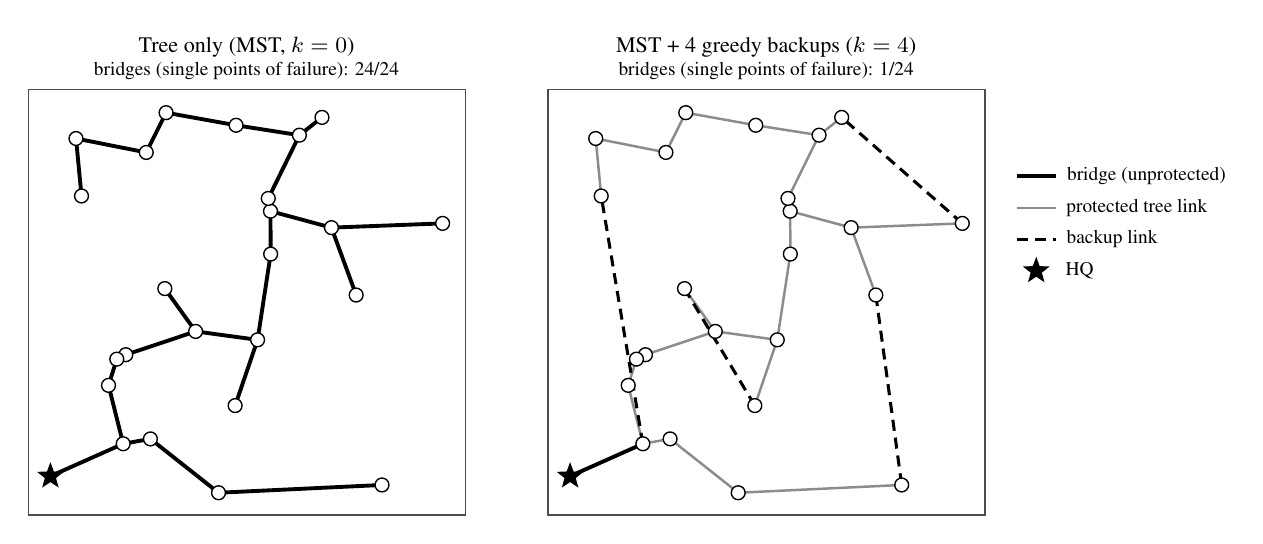
\begin{tikzpicture}
  \begin{scope}
    \draw[black!70,line width=0.5pt] (0.2,0.3) rectangle (5.75,5.7);
    \coordinate (n0) at (0.480,0.792);
\coordinate (n1) at (5.461,4.003);
\coordinate (n2) at (3.111,2.524);
\coordinate (n3) at (2.826,1.689);
\coordinate (n4) at (3.275,4.158);
\coordinate (n5) at (1.750,1.266);
\coordinate (n6) at (4.363,3.093);
\coordinate (n7) at (1.437,2.335);
\coordinate (n8) at (1.933,3.175);
\coordinate (n9) at (1.949,5.409);
\coordinate (n10) at (1.697,4.904);
\coordinate (n11) at (1.404,1.204);
\coordinate (n12) at (1.218,1.946);
\coordinate (n13) at (3.247,4.320);
\coordinate (n14) at (0.805,5.081);
\coordinate (n15) at (3.277,3.613);
\coordinate (n16) at (3.929,5.349);
\coordinate (n17) at (3.642,5.123);
\coordinate (n18) at (4.691,0.681);
\coordinate (n19) at (1.323,2.279);
\coordinate (n20) at (2.615,0.582);
\coordinate (n21) at (0.875,4.351);
\coordinate (n22) at (2.324,2.631);
\coordinate (n23) at (2.838,5.249);
\coordinate (n24) at (4.049,3.949);
\draw[bridge] (n7) -- (n19);
\draw[bridge] (n4) -- (n13);
\draw[bridge] (n12) -- (n19);
\draw[bridge] (n5) -- (n11);
\draw[bridge] (n16) -- (n17);
\draw[bridge] (n4) -- (n15);
\draw[bridge] (n9) -- (n10);
\draw[bridge] (n8) -- (n22);
\draw[bridge] (n14) -- (n21);
\draw[bridge] (n11) -- (n12);
\draw[bridge] (n2) -- (n22);
\draw[bridge] (n4) -- (n24);
\draw[bridge] (n17) -- (n23);
\draw[bridge] (n2) -- (n3);
\draw[bridge] (n13) -- (n17);
\draw[bridge] (n9) -- (n23);
\draw[bridge] (n10) -- (n14);
\draw[bridge] (n6) -- (n24);
\draw[bridge] (n7) -- (n22);
\draw[bridge] (n0) -- (n11);
\draw[bridge] (n2) -- (n15);
\draw[bridge] (n5) -- (n20);
\draw[bridge] (n1) -- (n24);
\draw[bridge] (n18) -- (n20);
\node[station] at (n1) {};
\node[station] at (n2) {};
\node[station] at (n3) {};
\node[station] at (n4) {};
\node[station] at (n5) {};
\node[station] at (n6) {};
\node[station] at (n7) {};
\node[station] at (n8) {};
\node[station] at (n9) {};
\node[station] at (n10) {};
\node[station] at (n11) {};
\node[station] at (n12) {};
\node[station] at (n13) {};
\node[station] at (n14) {};
\node[station] at (n15) {};
\node[station] at (n16) {};
\node[station] at (n17) {};
\node[station] at (n18) {};
\node[station] at (n19) {};
\node[station] at (n20) {};
\node[station] at (n21) {};
\node[station] at (n22) {};
\node[station] at (n23) {};
\node[station] at (n24) {};
\node[hq] at (n0) {};

    \node[paneltitle,above] at (2.97,5.7) {Tree only (MST, $k=0$)\\[-1pt]\normalfont\scriptsize bridges (single points of failure): 24/24};
  \end{scope}
  \begin{scope}[xshift=6.6cm]
    \draw[black!70,line width=0.5pt] (0.2,0.3) rectangle (5.75,5.7);
    \coordinate (n0) at (0.480,0.792);
\coordinate (n1) at (5.461,4.003);
\coordinate (n2) at (3.111,2.524);
\coordinate (n3) at (2.826,1.689);
\coordinate (n4) at (3.275,4.158);
\coordinate (n5) at (1.750,1.266);
\coordinate (n6) at (4.363,3.093);
\coordinate (n7) at (1.437,2.335);
\coordinate (n8) at (1.933,3.175);
\coordinate (n9) at (1.949,5.409);
\coordinate (n10) at (1.697,4.904);
\coordinate (n11) at (1.404,1.204);
\coordinate (n12) at (1.218,1.946);
\coordinate (n13) at (3.247,4.320);
\coordinate (n14) at (0.805,5.081);
\coordinate (n15) at (3.277,3.613);
\coordinate (n16) at (3.929,5.349);
\coordinate (n17) at (3.642,5.123);
\coordinate (n18) at (4.691,0.681);
\coordinate (n19) at (1.323,2.279);
\coordinate (n20) at (2.615,0.582);
\coordinate (n21) at (0.875,4.351);
\coordinate (n22) at (2.324,2.631);
\coordinate (n23) at (2.838,5.249);
\coordinate (n24) at (4.049,3.949);
\draw[protected] (n7) -- (n19);
\draw[protected] (n4) -- (n13);
\draw[protected] (n12) -- (n19);
\draw[protected] (n5) -- (n11);
\draw[protected] (n16) -- (n17);
\draw[protected] (n4) -- (n15);
\draw[protected] (n9) -- (n10);
\draw[protected] (n8) -- (n22);
\draw[protected] (n14) -- (n21);
\draw[protected] (n11) -- (n12);
\draw[protected] (n2) -- (n22);
\draw[protected] (n4) -- (n24);
\draw[protected] (n17) -- (n23);
\draw[protected] (n2) -- (n3);
\draw[protected] (n13) -- (n17);
\draw[protected] (n9) -- (n23);
\draw[protected] (n10) -- (n14);
\draw[protected] (n6) -- (n24);
\draw[protected] (n7) -- (n22);
\draw[bridge] (n0) -- (n11);
\draw[protected] (n2) -- (n15);
\draw[protected] (n5) -- (n20);
\draw[protected] (n1) -- (n24);
\draw[protected] (n18) -- (n20);
\draw[backup] (n11) -- (n21);
\draw[backup] (n6) -- (n18);
\draw[backup] (n3) -- (n8);
\draw[backup] (n1) -- (n16);
\node[station] at (n1) {};
\node[station] at (n2) {};
\node[station] at (n3) {};
\node[station] at (n4) {};
\node[station] at (n5) {};
\node[station] at (n6) {};
\node[station] at (n7) {};
\node[station] at (n8) {};
\node[station] at (n9) {};
\node[station] at (n10) {};
\node[station] at (n11) {};
\node[station] at (n12) {};
\node[station] at (n13) {};
\node[station] at (n14) {};
\node[station] at (n15) {};
\node[station] at (n16) {};
\node[station] at (n17) {};
\node[station] at (n18) {};
\node[station] at (n19) {};
\node[station] at (n20) {};
\node[station] at (n21) {};
\node[station] at (n22) {};
\node[station] at (n23) {};
\node[station] at (n24) {};
\node[hq] at (n0) {};

    \node[paneltitle,above] at (2.97,5.7) {MST + 4 greedy backups ($k=4$)\\[-1pt]\normalfont\scriptsize bridges (single points of failure): 1/24};
  \end{scope}
  \begin{scope}[xshift=12.75cm,yshift=3.4cm,font=\scriptsize]
    \draw[bridge] (0,1.2) -- (0.5,1.2) node[right,black] {bridge (unprotected)};
    \draw[protected] (0,0.8) -- (0.5,0.8) node[right,black] {protected tree link};
    \draw[backup] (0,0.4) -- (0.5,0.4) node[right,black] {backup link};
    \node[hq] at (0.25,0) {}; \node[right] at (0.5,0) {HQ};
  \end{scope}
\end{tikzpicture}
\caption{Backup links turn single-point bridges into protected cycles ($n=25$, Seed~7, regenerated from the
Mulberry32 stream). Left: the MST leaves all 24/24 tree edges as vulnerable bridges (heavy solid). Right: $k=4$ greedy
backups (dashed) close long fundamental cycles, turning 23 tree edges into protected cycle edges (light solid) and leaving a
single leaf bridge at HQ.}
\label{fig:bridges}
\end{figure}

\begin{keybox}{Link failures versus station failures}
An individual \textbf{link failure} deletes one edge $e$ while all stations remain online. A \textbf{station failure}
deletes vertex $v$ and \emph{all incident tree and backup links simultaneously}. Protecting every tree edge with a cycle
guarantees 2-edge-connectivity (survival of any single link cut) but does \textbf{not} eliminate articulation vertices---for
example, two cycles sharing a single hub station. Both regimes are tested explicitly in Section~\ref{sec:outage}.
\end{keybox}

% ==================================================================
\section{Submodular Backup Cycle Coverage}\label{sec:coverage}

\subsection{Fundamental cycles and edge protection}
To protect $T$ against single-link cuts with at most $k$ backups $S\subseteq L=E_0\setminus E_T$, observe that adding a
candidate $\ell=(u,v)\in L$ closes a unique fundamental cycle $P_\ell\cup\{\ell\}$, where $P_\ell\subseteq E_T$ is the tree
path between $u$ and $v$. The design problem is
\begin{equation}\label{eq:cov}
  \mathrm{Cov}(S)=\bigcup_{\ell\in S}P_\ell,\qquad
  F(S)=\sum_{e\in\mathrm{Cov}(S)}w_e,\qquad
  \max_{S\subseteq L,\;|S|\le k} F(S).
\end{equation}

\begin{lemma}[Protection of a tree edge]\label{lem:protect}
For any tree edge $e\in E_T$, the augmented graph $G-e$ remains connected if and only if $e\in\mathrm{Cov}(S)$.
\end{lemma}
\begin{proof}
Removing $e$ partitions $T$ into two subtrees $T_1,T_2$. A backup $\ell=(u,v)\in S$ reconnects them if and only if its
endpoints lie in opposite subtrees, which holds if and only if the unique tree path $P_\ell$ crosses the cut edge, i.e.\
$e\in P_\ell$. Taking the union over $\ell\in S$, $G-e$ stays connected if and only if $e\in\mathrm{Cov}(S)$.
\end{proof}

\subsection{Diminishing returns and the greedy guarantee}
Adding a backup $\ell$ to a selection $A\subseteq L$ yields the exact marginal gain
\begin{equation}\label{eq:gain}
  F(A\cup\{\ell\})-F(A)=\sum_{e\in P_\ell\setminus\mathrm{Cov}(A)}w_e .
\end{equation}

\begin{proposition}\label{prop:submod}
$F$ is normalized ($F(\emptyset)=0$), monotone nondecreasing and submodular on $2^L$.
\end{proposition}
\begin{proof}
Normalization and monotonicity follow from $w_e\ge0$ and $\mathrm{Cov}(A)\subseteq\mathrm{Cov}(A\cup\{\ell\})$. For
$A\subseteq B\subseteq L$ we have $\mathrm{Cov}(A)\subseteq\mathrm{Cov}(B)$, so the uncovered part of the path shrinks,
$P_\ell\setminus\mathrm{Cov}(B)\subseteq P_\ell\setminus\mathrm{Cov}(A)$, and by Eq.~\eqref{eq:gain} with $w_e\ge0$,
$F(A\cup\{\ell\})-F(A)\ge F(B\cup\{\ell\})-F(B)$.
\end{proof}

\begin{theorem}[Nemhauser--Wolsey--Fisher~\cite{nemhauser}]\label{thm:greedy}
Let $S_g$ be the set returned by $k$ steps of exact marginal-gain greedy selection and $S^\ast$ an optimal solution of
\eqref{eq:cov}. Then
\begin{equation}\label{eq:bound}
  F(S_g)\;\ge\;\Bigl[1-\bigl(1-\tfrac1k\bigr)^{k}\Bigr]F(S^\ast)\;\ge\;\bigl(1-\tfrac1e\bigr)F(S^\ast)\;\approx\;0.632\,F(S^\ast).
\end{equation}
\end{theorem}
\begin{proof}
Let $S_t$ be the greedy set after $t$ steps. By monotonicity and submodularity,
\begin{equation}\label{eq:gap}
  F(S^\ast)-F(S_t)\;\le\;\sum_{\ell\in S^\ast\setminus S_t}\bigl[F(S_t\cup\{\ell\})-F(S_t)\bigr].
\end{equation}
Since $|S^\ast\setminus S_t|\le k$, the best next greedy choice captures at least a $1/k$ fraction of the remaining gap,
$F(S^\ast)-F(S_{t+1})\le(1-1/k)\,[F(S^\ast)-F(S_t)]$. Iterating $k$ times from $F(S_0)=0$ gives \eqref{eq:bound}.
\end{proof}

By Lemma~\ref{lem:protect}, $F(S)$ with unit weights counts exactly the tree links that survive any single cut, so
Theorem~\ref{thm:greedy} is a resilience guarantee. Figure~\ref{fig:greedy} compares greedy with the exhaustive optimum.
On average greedy is indistinguishable from optimal and far above both random selection and the worst case the theorem
allows; across 900 scenarios it attains the optimum in 871 (96.78\%), with worst ratio 0.875---well above the 0.632 floor.

\begin{figure}[t]
\centering
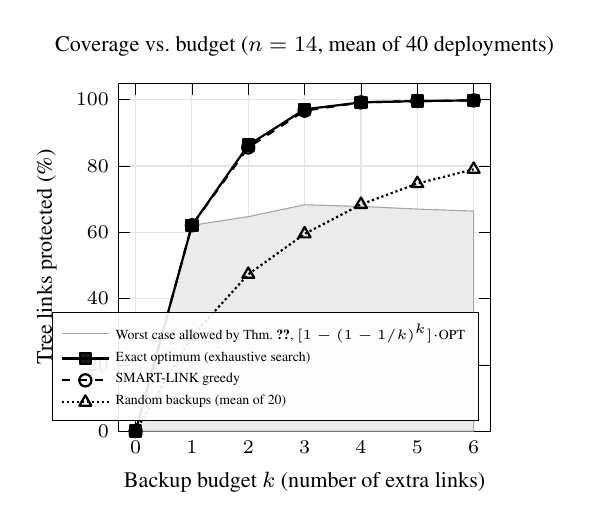
\begin{tikzpicture}
\begin{axis}[width=0.52\textwidth,height=6.0cm,
  title={Coverage vs.\ budget ($n=14$, mean of 40 deployments)},
  xlabel={Backup budget $k$ (number of extra links)}, ylabel={Tree links protected (\%)},
  xmin=-0.3,xmax=6.3,ymin=0,ymax=105,xtick={0,...,6},ytick={0,20,...,100},
  legend pos=south east, legend style={font=\tiny}]
  \addplot[fill=black!8,draw=black!35] coordinates {(0,0)(1,62.1)(2,64.7)(3,68.3)(4,67.8)(5,67.0)(6,66.4)(6,0)} \closedcycle;
  \addlegendentry{Worst case allowed by Thm.~\ref{thm:greedy}, $[1-(1-1/k)^k]\cdot$OPT}
  \addplot[black,thick,mark=square*,mark size=2pt] coordinates {(0,0)(1,62.1)(2,86.3)(3,97.1)(4,99.2)(5,99.6)(6,99.8)};
  \addlegendentry{Exact optimum (exhaustive search)}
  \addplot[black,thick,dashed,mark=o,mark size=2.2pt,mark options={solid}] coordinates {(0,0)(1,62.1)(2,85.6)(3,96.7)(4,99.2)(5,99.6)(6,99.8)};
  \addlegendentry{SMART-LINK greedy}
  \addplot[black,thick,densely dotted,mark=triangle,mark size=2.5pt,mark options={solid}] coordinates {(0,0)(1,28.6)(2,47.3)(3,59.5)(4,68.4)(5,74.7)(6,79.0)};
  \addlegendentry{Random backups (mean of 20)}
\end{axis}
\end{tikzpicture}\hfill
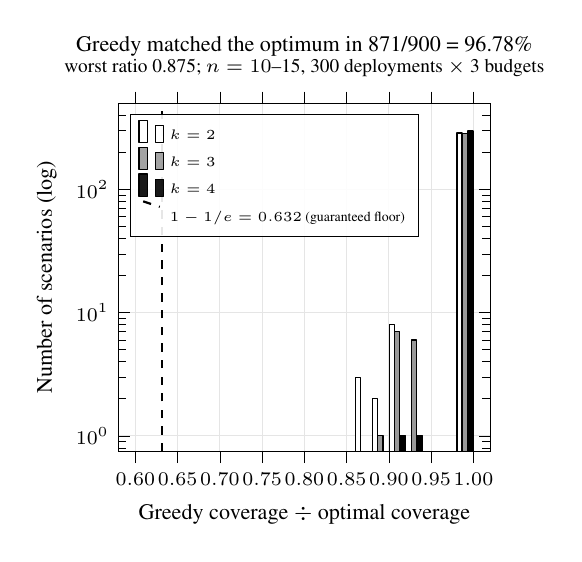
\begin{tikzpicture}
\begin{axis}[width=0.52\textwidth,height=6.0cm,
  title={Greedy matched the optimum in 871/900 = 96.78\%\\[-2pt]\normalfont\scriptsize worst ratio 0.875; $n=10$--15, 300 deployments $\times$ 3 budgets},
  xlabel={Greedy coverage $\div$ optimal coverage}, ylabel={Number of scenarios (log)},
  ymode=log, log origin=infty, xmin=0.58, xmax=1.02, ymin=0.75, ymax=500,
  xtick={0.6,0.65,...,1.0}, xticklabel style={/pgf/number format/.cd,fixed,precision=2,fixed zerofill},
  ybar, bar width=0.006, legend pos=north west, legend style={font=\tiny}]
  \addplot[fill=white,draw=black,bar shift=-0.0065] coordinates {(0.87,3)(0.89,2)(0.91,8)(0.99,287)};
  \addlegendentry{$k=2$}
  \addplot[fill=black!40,draw=black,bar shift=0] coordinates {(0.89,1)(0.91,7)(0.93,6)(0.99,286)};
  \addlegendentry{$k=3$}
  \addplot[fill=black,draw=black,bar shift=0.0065] coordinates {(0.91,1)(0.93,1)(0.99,298)};
  \addlegendentry{$k=4$}
  \addplot[sharp plot,black,thick,dashed] coordinates {(0.632,0.75)(0.632,500)};
  \addlegendentry{$1-1/e=0.632$ (guaranteed floor)}
\end{axis}
\end{tikzpicture}
\caption{Greedy backup selection versus the exact optimum. Left: mean percentage of tree edges protected versus budget
$k\in\{0,\dots,6\}$ over 40 deployments ($n=14$), compared with random selection and the theoretical floor. Right:
distribution of the greedy/optimal ratio over 900 benchmark scenarios ($n\in[10,15]$, $k\in\{2,3,4\}$).}
\label{fig:greedy}
\end{figure}

% ==================================================================
\section{From the Hadwiger--Nelson Problem to Spectrum Assignment}\label{sec:spectrum}

\subsection{Plane colouring and hexagonal reuse}
The investigation began with the classical Hadwiger--Nelson problem: what is the least number of colours $\chi(\mathbb R^2)$
needed to colour the plane so that no two points at unit distance share a colour? It is known that
$5\le\chi(\mathbb R^2)\le7$, the lower bound being due to de~Grey (2018). Isbell's upper-bound construction tiles the plane
with regular hexagons of diameter slightly below 1 in a periodic 7-colour pattern---and that tiling is precisely the
geometry of cellular frequency reuse. Valid hexagonal cluster sizes are $N=i^2+ij+j^2\in\{1,3,4,7,9,12,13,\dots\}$; the choice
$i=2$, $j=1$ gives the canonical $N=7$ cluster with co-channel reuse distance $D=R\sqrt{3N}=\sqrt{21}\,R\approx4.58R$.
With path-loss exponent $\gamma=4$ and six first-tier interferers the worst-case signal-to-interference ratio is
$\mathrm{SIR}\approx(\sqrt{3N})^4/6=441/6=73.5$ (18.66\,dB), above the classic 18\,dB threshold (Fig.~\ref{fig:hex}).

\begin{figure}[t]
\centering
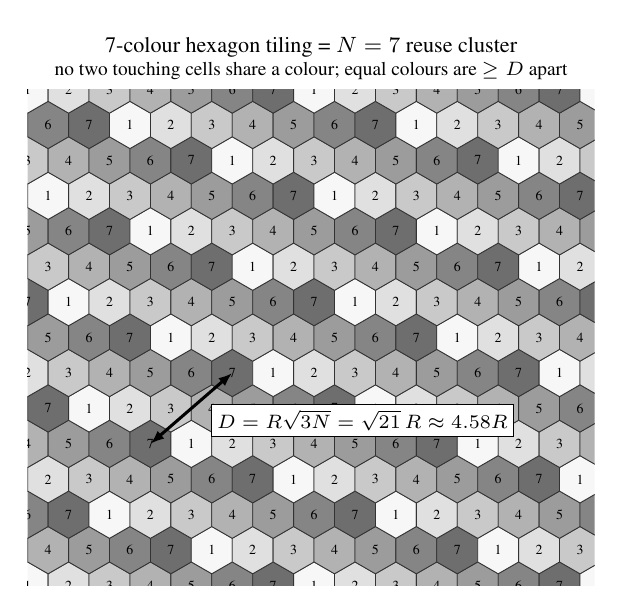
\begin{tikzpicture}
  \def\R{0.3}
  \begin{scope}
    \clip (0,0) rectangle (7.2,6.3);
    \foreach \r in {-1,...,15}{
      \foreach \q in {-10,...,16}{
        \pgfmathsetmacro\cx{sqrt(3)*\R*(\q+\r/2)}
        \pgfmathsetmacro\cy{1.5*\R*\r}
        \pgfmathtruncatemacro\c{mod(mod(\q+3*\r,7)+7,7)}
        \pgfmathtruncatemacro\lab{\c+1}
        \ifdim\cx pt>-0.6pt\ifdim\cx pt<7.8pt
          \filldraw[fill=hc\c,draw=black!80,line width=0.3pt,shift={(\cx,\cy)}]
            (90:\R) -- (150:\R) -- (210:\R) -- (270:\R) -- (330:\R) -- (30:\R) -- cycle;
          \node[font=\tiny] at (\cx,\cy) {\lab};
        \fi\fi
      }
    }
  \end{scope}
  % co-channel pair: axial (q,r)=(1,4) and (2,6) differ by (1,2), so both carry channel 7, sqrt(7) cell spacings apart
  \pgfmathsetmacro\ax{sqrt(3)*\R*(1+4/2)}\pgfmathsetmacro\ay{1.5*\R*4}
  \pgfmathsetmacro\bx{sqrt(3)*\R*(2+6/2)}\pgfmathsetmacro\by{1.5*\R*6}
  \draw[{Latex[length=5pt]}-{Latex[length=5pt]},line width=1.1pt] (\ax,\ay) -- (\bx,\by);
  \node[draw=black,fill=white,font=\scriptsize,inner sep=2pt,anchor=west] at ($(\ax,\ay)!0.5!(\bx,\by)+(0.25,-0.15)$) {$D=R\sqrt{3N}=\sqrt{21}\,R\approx4.58R$};
  \node[paneltitle,above] at (3.6,6.3) {7-colour hexagon tiling = $N=7$ reuse cluster\\[-1pt]\normalfont\scriptsize no two touching cells share a colour; equal colours are $\ge D$ apart};
\end{tikzpicture}\hfill
\begin{tikzpicture}[baseline={(0,0)}]
\begin{axis}[width=0.5\textwidth,height=6.6cm,
  title={More carriers per cluster $\rightarrow$ cleaner signal\\[-1pt]\normalfont\scriptsize SIR $\approx(\sqrt{3N})^4/6$, path-loss exponent 4},
  xlabel={Cluster size $N=i^2+ij+j^2$ (carriers needed)}, ylabel={Worst-case SIR (dB)},
  xmin=0,xmax=22,ymin=0,ymax=30,
  nodes near coords={\tiny\pgfmathprintnumber{\pgfplotspointmeta}}, point meta=x,
  every node near coord/.append style={anchor=south,yshift=1pt}]
  \addplot[black,thick,mark=*,mark size=2pt] table[x=N,y=sir] {data/sir.dat};
  \addplot[black,thick,dashed,nodes near coords={}] coordinates {(0,18)(22,18)};
  \node[font=\tiny,anchor=north] at (axis cs:16.5,17.4) {18\,dB target (classic AMPS)};
\end{axis}
\end{tikzpicture}
\caption{From Hadwiger--Nelson to frequency reuse. Left: Isbell's 7-colour hexagonal tiling (the upper bound
$\chi(\mathbb R^2)\le7$) coincides with the $N=7$ reuse cluster, here shaded by channel $(q+3r)\bmod 7$ in axial
coordinates; co-channel cells are $D=R\sqrt{3N}\approx4.58R$ apart. Right: first-tier SIR across valid cluster sizes
under $\gamma=4$; point labels give $N$.}
\label{fig:hex}
\end{figure}

\subsection{Why point-to-point relays collide}
Disaster networks depart from the ideal lattice in two ways: stations are placed irregularly by terrain, and
connections are directional point-to-point \emph{links} rather than omnidirectional cells. If two links meeting at a
relay transmit and receive on the same carrier simultaneously, the station's own $+30$\,dBm (1\,W) transmission is
140\,dB---$10^{14}$ times---stronger than a faint incoming signal near the $-110$\,dBm thermal floor, and drowns it.
Without multi-channel planning, narrowband radios fall back to half-duplex TDMA: station~1 sends in slot~1 (0--20\,ms) while
station~2 buffers, and station~2 forwards in slot~2 (20--40\,ms). Over long backbones, store-and-forward turn-taking
compounds queuing latency at every hop. Separating conflicting links \emph{in frequency} removes the contention.

\subsection{The link conflict graph}
Because carriers are assigned to links $e\in E=E_T\cup S$ rather than to towers, SMART-LINK maps $G=(V,E)$ to a conflict
graph $H_c=(E,I)$ whose vertices are links. With $m_e=(p_u+p_v)/2$ the midpoint of $e=(u,v)$, two distinct links conflict if
\begin{equation}\label{eq:conflict}
  A_{e,e'}=\begin{cases}
    1 & \text{if } e\cap e'\neq\emptyset \text{ (station incidence), or spatial mode is on and } \|m_e-m_{e'}\|_2\le R_I,\\
    0 & \text{otherwise.}\end{cases}
\end{equation}
With station-incidence conflicts alone, $H_c$ is the line graph $L(G)$ and Vizing's theorem~\cite{vizing} bounds the
edge-chromatic number by $\Delta(G)\le\chi'(G)\le\Delta(G)+1$. Spatial conflicts (default $R_I=0.04$), per-link jammed-carrier
exclusions and a minimum centre spacing turn the problem into list-constrained $T$-colouring on a supergraph of $L(G)$:
\begin{align}
  f_e\in L_e=\mathcal F\setminus J_e,\qquad |f_e-f_{e'}|&\ge s \quad\text{for every }\{e,e'\}\in I, \label{eq:sep}\\
  |f_e-f_{e'}|&\ge \tfrac{B_e+B_{e'}}{2}+g_{e,e'}. \label{eq:guard}
\end{align}
SMART-LINK orders links by nonincreasing conflict degree in $H_c$ (ties broken by endpoint IDs) and gives each the lowest
carrier in $L_e$ that is at least $s$ from all already-assigned conflicting neighbours, flagging any link that cannot be
assigned. Figure~\ref{fig:spectrum} shows the bit-exact Seed-42 result and a jamming stress test.

\begin{figure}[t]
\centering
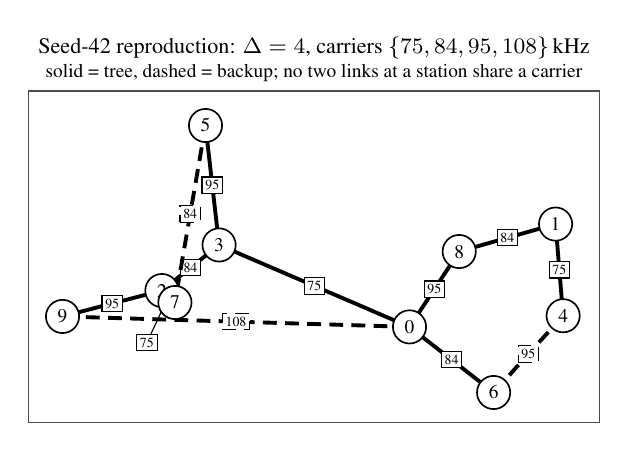
\begin{tikzpicture}[scale=0.78]
  \draw[black!70,line width=0.5pt] (0.25,2.55) rectangle (9.55,7.95);
  \coordinate (n0) at (6.456,4.109);
\coordinate (n1) at (8.834,5.783);
\coordinate (n2) at (2.424,4.701);
\coordinate (n3) at (3.355,5.443);
\coordinate (n4) at (8.957,4.291);
\coordinate (n5) at (3.134,7.388);
\coordinate (n6) at (7.825,3.041);
\coordinate (n7) at (2.636,4.506);
\coordinate (n8) at (7.265,5.336);
\coordinate (n9) at (0.806,4.279);
\draw[tree42,draw=c75] (n2) -- (n7);
\node[carrier,draw=c75] (lab27) at ($(n2)!0.5!(n7)+(-0.35,-0.75)$) {75};
\draw[c75,thin] (lab27) -- ($(n2)!0.5!(n7)$);
\draw[tree42,draw=c84] (n2) -- node[carrier,draw=c84] {84} (n3);
\draw[tree42,draw=c84] (n1) -- node[carrier,draw=c84] {84} (n8);
\draw[tree42,draw=c95] (n2) -- node[carrier,draw=c95] {95} (n9);
\draw[tree42,draw=c95] (n0) -- node[carrier,draw=c95] {95} (n8);
\draw[tree42,draw=c75] (n1) -- node[carrier,draw=c75] {75} (n4);
\draw[tree42,draw=c84] (n0) -- node[carrier,draw=c84] {84} (n6);
\draw[tree42,draw=c95] (n3) -- node[carrier,draw=c95] {95} (n5);
\draw[tree42,draw=c75] (n0) -- node[carrier,draw=c75] {75} (n3);
\draw[backup42,draw=c95] (n4) -- node[carrier,draw=c95] {95} (n6);
\draw[backup42,draw=c84] (n5) -- node[carrier,draw=c84] {84} (n7);
\draw[backup42,draw=c108] (n0) -- node[carrier,draw=c108] {108} (n9);
\node[station42] at (n0) {0};
\node[station42] at (n1) {1};
\node[station42] at (n2) {2};
\node[station42] at (n3) {3};
\node[station42] at (n4) {4};
\node[station42] at (n5) {5};
\node[station42] at (n6) {6};
\node[station42] at (n7) {7};
\node[station42] at (n8) {8};
\node[station42] at (n9) {9};

  \node[paneltitle,above] at (4.9,7.95) {Seed-42 reproduction: $\Delta=4$, carriers $\{75,84,95,108\}$\kHz\\[-1pt]\normalfont\scriptsize solid = tree, dashed = backup; no two links at a station share a carrier};
\end{tikzpicture}\hfill
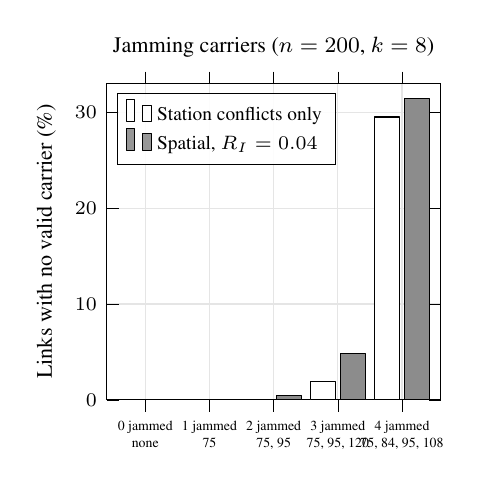
\begin{tikzpicture}
\begin{axis}[width=0.48\textwidth,height=5.6cm,
  title={Jamming carriers ($n=200$, $k=8$)},
  ylabel={Links with no valid carrier (\%)},
  ybar, bar width=9pt, ymin=0, ymax=33, xtick={0,...,4}, xmin=-0.6, xmax=4.6,
  xticklabels={{0 jammed\\none},{1 jammed\\75},{2 jammed\\75, 95},{3 jammed\\75, 95, 120},{4 jammed\\75, 84, 95, 108}},
  xticklabel style={align=center,font=\tiny}, legend pos=north west]
  \addplot[fill=white,draw=black] coordinates {(0,0)(1,0)(2,0)(3,1.9)(4,29.5)};
  \addlegendentry{Station conflicts only}
  \addplot[fill=black!45,draw=black] coordinates {(0,0)(1,0)(2,0.5)(3,4.8)(4,31.4)};
  \addlegendentry{Spatial, $R_I=0.04$}
\end{axis}
\end{tikzpicture}
\caption{Conflict-aware carrier assignment. Left: bit-exact reproduction of the Seed-42 ten-station baseline ($k=3$):
nine tree links (solid) and three backups (dashed) coloured with four carriers, the provable minimum since $\Delta(G)=4$.
Right: a 200-station network ($k=8$) as an adversary jams 0--4 of the six raster carriers, under station-only and spatial
conflict modes.}
\label{fig:spectrum}
\end{figure}

\begin{keybox}{Centre spacing $s$ is not an empty guard band}
In Eq.~\eqref{eq:guard}, $s=9$\kHz\ is a \emph{centre-to-centre} spacing, not a 9\kHz\ gap. If neighbouring links occupy
$B_e=B_{e'}=4$\kHz, then $(B_e+B_{e'})/2=4$\kHz\ is filled by signal sidebands, leaving an unoccupied guard band
$g_{e,e'}=9-4=5$\kHz\ for filter roll-off.
\end{keybox}

% ==================================================================
\section{Inside the Relay: Heterodyne Mixing and Filter Delay}\label{sec:relay}

\subsection{Product-to-sum frequency translation}
Suppose colouring assigns the incoming link (station~1 $\to$ relay~2) to $f_\text{in}=95$\kHz\ and the outgoing link
(relay~2 $\to$ station~3) to $f_\text{out}=75$\kHz. An analog heterodyne relay shifts the carrier without decrypting the
payload. Let $s_\text{in}(t)=a(t)\cos(2\pi f_\text{in}t+\phi(t))$ and multiply by a local oscillator
$s_\text{LO}(t)=2\cos(2\pi f_\text{LO}t)$ with $f_\text{LO}=20$\kHz. The identity $2\cos A\cos B=\cos(A-B)+\cos(A+B)$ gives
\begin{equation}\label{eq:mix}
  y_\text{mix}(t)=a(t)\cos\bigl(2\pi(f_\text{in}-f_\text{LO})t+\phi(t)\bigr)+a(t)\cos\bigl(2\pi(f_\text{in}+f_\text{LO})t+\phi(t)\bigr),
\end{equation}
i.e.\ $Y_\text{mix}(f)=S_\text{in}(f-f_\text{LO})+S_\text{in}(f+f_\text{LO})$, where the factor 2 in $s_\text{LO}$ preserves unit
passband amplitude. Mixing therefore produces the wanted difference carrier at 75\kHz\ and an unwanted sum image at
115\kHz, which a band-pass filter must remove (Fig.~\ref{fig:fft}).

\begin{figure}[t]
\centering
\begin{tikzpicture}
\begin{groupplot}[group style={group size=1 by 3,vertical sep=0.95cm,xticklabels at=edge bottom},
  width=\textwidth,height=3.9cm,xmin=0,xmax=160,ymin=-120,ymax=10,ytick={-120,-100,...,0},
  ylabel={dB},unbounded coords=jump,every axis title/.append style={font=\scriptsize,yshift=-3pt}]
  \nextgroupplot[title={Received signal at relay (95\kHz\ carrier)}]
    \foreach \f in {75,95,115}{\edef\tmp{\noexpand\draw[gray,densely dotted] (axis cs:\f,-120) -- (axis cs:\f,10);}\tmp}
    \addplot[black,line width=0.5pt] table[x=f,y=db] {data/fft_in.dat};
  \nextgroupplot[title={After mixing with the 20\kHz\ local oscillator}]
    \foreach \f in {75,95,115}{\edef\tmp{\noexpand\draw[gray,densely dotted] (axis cs:\f,-120) -- (axis cs:\f,10);}\tmp}
    \addplot[black,line width=0.5pt] table[x=f,y=db] {data/fft_mix.dat};
    \draw[-{Latex[length=4pt]}] (axis cs:57,-20) node[below,font=\scriptsize]{75\kHz\ (wanted)} -- (axis cs:74,-1);
    \draw[-{Latex[length=4pt]}] (axis cs:133,-20) node[below,font=\scriptsize]{115\kHz\ (unwanted image)} -- (axis cs:116,-1);
  \nextgroupplot[title={After 6th-order Butterworth band-pass 73--77\kHz\ (transmitted)},xlabel={Frequency (kHz)}]
    \foreach \f in {75,95,115}{\edef\tmp{\noexpand\draw[gray,densely dotted] (axis cs:\f,-120) -- (axis cs:\f,10);}\tmp}
    \addplot[black,line width=0.5pt] table[x=f,y=db] {data/fft_out.dat};
    \node[font=\scriptsize,align=left,anchor=west] at (axis cs:118,-35) {115\kHz\ image suppressed by\\$\approx$74\,dB relative to 75\kHz};
\end{groupplot}
\end{tikzpicture}
\caption{FFT verification of Eq.~\eqref{eq:mix} (65{,}536 samples, $f_s=1$\,MS/s, Blackman window; recomputed natively).
Top: incoming 95\kHz\ carrier amplitude-modulated by a 500\,Hz tone. Middle: mixer output with equal-amplitude products at
75 and 115\kHz. Bottom: after the 73--77\kHz\ Butterworth band-pass, the 75\kHz\ signal passes and the 115\kHz\ image is
suppressed by 74.3\,dB.}
\label{fig:fft}
\end{figure}

\subsection{Adjacent-channel rejection and group delay}
Filter rejection and group delay must be measured rather than assumed. Evaluating the 6th-order (order-3 band-pass
prototype) Butterworth filter with \texttt{scipy.signal.sosfreqz} and its phase derivative establishes:
\begin{itemize}\setlength\itemsep{1pt}
  \item \textbf{Adjacent-carrier rejection:} 37.9\,dB at the nearest raster neighbour (84\kHz), 57.4\,dB at 95\kHz,
        69.3\,dB at 108\kHz, and 73.8--74.3\,dB at the 115\kHz\ sum image.
  \item \textbf{Non-zero group delay:} any causal, sharp band-pass filter stores energy in its reactive stages. At 75\kHz\
        the group delay is $\tau_g=159.1$\us\ per relay hop, peaking above 200\us\ near the 73 and 77\kHz\ band edges. Analog
        translation is thus $\approx$125$\times$ faster than a 20\,ms TDMA slot, but not instantaneous (Fig.~\ref{fig:filter}).
\end{itemize}

\begin{figure}[t]
\centering
\begin{tikzpicture}
\begin{axis}[width=0.47\textwidth,height=5.4cm,title={Band-pass magnitude response},
  xlabel={Frequency (kHz)},ylabel={Gain (dB)},xmin=50,xmax=130,ymin=-100,ymax=5]
  \addplot[black,thick] table[x=f,y=g] {data/bp_mag.dat};
  \addplot[only marks,mark=*,mark size=1.8pt,black,
    nodes near coords={\tiny\pgfmathprintnumber[fixed,precision=0]{\pgfkeysvalueof{/data point/x}}k\\[-3pt]\tiny$\pgfmathprintnumber[fixed,precision=0]{\pgfplotspointmeta}$\,dB},
    point meta=y, every node near coord/.append style={anchor=north,align=center,text=black,yshift=-1pt}]
    table[x=f,y=g] {data/bp_pts.dat};
\end{axis}
\end{tikzpicture}\hfill
\begin{tikzpicture}
\begin{axis}[width=0.47\textwidth,height=5.4cm,title={Group delay $\approx$ 159\us\ at 75\kHz\ (per relay)},
  xlabel={Frequency (kHz)},ylabel={Group delay (\textmu s)},xmin=64,xmax=86,ymin=-5,ymax=235,
  xticklabel style={/pgf/number format/.cd,fixed,precision=1,fixed zerofill}]
  \addplot[black,thick] table[x=f,y=gd] {data/bp_gd.dat};
  \addplot[black,densely dashed] coordinates {(75,-5)(75,235)};
\end{axis}
\end{tikzpicture}
\caption{The relay filter is not instantaneous. Left: magnitude response of the 6th-order 73--77\kHz\ Butterworth band-pass
with attenuation at neighbouring raster frequencies. Right: passband group delay (159.1\us\ at 75\kHz), the physical filter
latency added at each hop.}
\label{fig:filter}
\end{figure}

% ==================================================================
\section{Physical-Layer RF Analysis}\label{sec:rf}

Full-duplex and multi-link operation depend on residual transmitter leakage and on the
signal-to-interference-plus-noise ratio,
\begin{equation}\label{eq:leak}
  P_\text{residual}=P_\text{tx}-A_\text{antenna}-A_\text{filter}-A_\text{cancellation}\quad\text{(dBm, dB)},
\end{equation}
\begin{equation}\label{eq:sinr}
  \mathrm{SINR}_e=\frac{P_e\,g_e}{N_0B_e+\sum_{j\neq e}P_j\,g_{j\to e}\,\eta_{j,e}},\qquad C_e=B_e\log_2(1+\mathrm{SINR}_e).
\end{equation}
To keep narrowband low-IF benchmarks distinct from wideband tactical-radio specifications, we ran four quantitative
evaluations (Figs.~\ref{fig:bpsk} and~\ref{fig:rf}).

\paragraph{Passband data-rate ceiling.} By the Shannon limit in Eq.~\eqref{eq:sinr}, a 4\kHz\ filter cannot carry wideband
128\,kbit/s or 16\,Mbit/s waveforms: 128\,kbit/s in 9\kHz\ already needs $\mathrm{SINR}\ge42.8$\,dB, and 16\,Mbit/s needs
megahertz of UHF/SHF spectrum. Sweeping BPSK symbol rates through the 73--77\kHz\ filter gives 0\% bit errors up to
8\,kbit/s, then severe inter-symbol interference (20.4\% BER at 12\,kbit/s) once symbol bandwidth exceeds the passband.

\paragraph{Amplify-and-forward noise.} Unlike decode-and-forward relays, which regenerate clean bits, analog heterodyne
relays amplify incoming thermal noise at every stage. Over $h$ identical hops of per-hop SNR$_1$,
$\mathrm{SNR}_{\text{total,dB}}=\mathrm{SNR}_{1,\text{dB}}-10\log_{10}h$: 10\,dB lost over 10 hops, 20\,dB over 100.

\paragraph{Quarter-wave antenna scaling.} At 75\kHz\ (LF, $\lambda=c/f=4{,}000$\,m) a quarter-wave whip is
$\lambda/4=1{,}000$\,m tall. The 75--135\kHz\ raster is therefore a mathematical raster or internal IF/ultrasonic test stage;
field radios up-convert to 433\,MHz LoRa/ISM ($\lambda/4=17.3$\,cm) or 2.4\,GHz ($\lambda/4=3.1$\,cm).

\paragraph{Same-band full-duplex leakage.} With $P_\text{tx}=+30$\,dBm and 85\,dB aggregate suppression, Eq.~\eqref{eq:leak}
leaves $P_\text{residual}=-55$\,dBm---still 55\,dB above a $-110$\,dBm noise floor. Reaching the floor needs 140\,dB total
isolation~\cite{bharadia,smida}, or frequency-separated FDD across distinct carriers.

\begin{figure}[t]
\centering
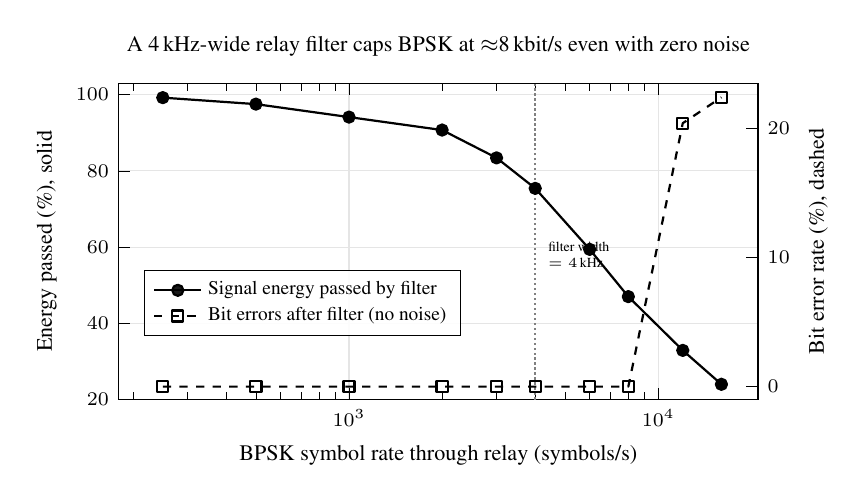
\begin{tikzpicture}
\begin{axis}[width=0.8\textwidth,height=5.6cm,xmode=log,xmin=180,xmax=21000,ymin=20,ymax=103,
  axis y line*=left, ylabel={Energy passed (\%), solid}, xlabel={BPSK symbol rate through relay (symbols/s)},
  title={A 4\kHz-wide relay filter caps BPSK at $\approx$8\,kbit/s even with zero noise},
  legend style={at={(0.04,0.2)},anchor=south west}]
  \addplot[black,thick,mark=*,mark size=2pt] coordinates {(250,99.2)(500,97.5)(1000,94.1)(2000,90.7)(3000,83.4)(4000,75.4)(6000,59.4)(8000,47.0)(12000,32.9)(16000,24.0)};
  \addlegendentry{Signal energy passed by filter}
  \addlegendimage{black,thick,dashed,mark=square,mark options={solid}}
  \addlegendentry{Bit errors after filter (no noise)}
  \draw[gray,thick,densely dotted] (axis cs:4000,20) -- (axis cs:4000,103);
  \node[font=\tiny,anchor=south west,align=left] at (axis cs:4100,52) {filter width\\$=4$\kHz};
\end{axis}
\begin{axis}[width=0.8\textwidth,height=5.6cm,xmode=log,xmin=180,xmax=21000,ymin=-1,ymax=23.5,
  axis y line*=right, axis x line=none, grid=none, ylabel={Bit error rate (\%), dashed}]
  \addplot[black,thick,dashed,mark=square,mark size=2pt,mark options={solid}] coordinates {(250,0)(500,0)(1000,0)(2000,0)(3000,0)(4000,0)(6000,0)(8000,0)(12000,20.4)(16000,22.4)};
\end{axis}
\end{tikzpicture}
\caption{BPSK symbol-rate sweep through the 6th-order 73--77\kHz\ (4\kHz) Butterworth band-pass with delay-correlation
synchronization: error-free up to 8\,kbit/s, sideband clipping above 10\,kbit/s. The 128\,kbit/s and 16\,Mbit/s
channels sometimes quoted for such links cannot fit.}
\label{fig:bpsk}
\end{figure}

\begin{figure}[tbp]
\centering
\begin{tikzpicture}
\begin{groupplot}[group style={group size=2 by 2,horizontal sep=1.8cm,vertical sep=2.3cm},width=0.5\textwidth,height=6.3cm]
  % A ---------------------------------------------------------
  \nextgroupplot[title={A.\ Maximum data rate in a narrow slot\\[-1pt]\normalfont\scriptsize 128\,kbit/s needs SNR $\ge$ 43\,dB in 9\kHz; 16\,Mbit/s is impossible},
    xlabel={Signal-to-noise ratio (dB)},ylabel={bit/s},ymode=log,ymin=1e3,ymax=1e8,xmin=-3,xmax=63,
    legend pos=south east]
    \addplot[black,thick] table[x=snr,y=c4] {data/shannon.dat}; \addlegendentry{Shannon limit, $B=4$\kHz}
    \addplot[black,thick,dashed] table[x=snr,y=c9] {data/shannon.dat}; \addlegendentry{Shannon limit, $B=9$\kHz}
    \addplot[black,densely dotted,forget plot] coordinates {(-3,1.6e7)(63,1.6e7)};
    \addplot[black,densely dotted,forget plot] coordinates {(-3,1.28e5)(63,1.28e5)};
    \node[font=\scriptsize,anchor=south west] at (axis cs:0,1.6e7) {claimed 16\,Mbit/s};
    \node[font=\scriptsize,anchor=south west] at (axis cs:0,1.28e5) {claimed 128\,kbit/s};
  % B ---------------------------------------------------------
  \nextgroupplot[title={B.\ Amplify-and-forward relays add noise every hop\\[-1pt]\normalfont\scriptsize dotted = decode-and-forward (regenerates signal, needs buffering)},
    xlabel={Number of relay hops},ylabel={End-to-end SNR (dB)},xmin=-4,xmax=124,ymin=-3,ymax=42,
    legend style={font=\tiny},legend pos=north east]
    \addplot[black,thick] table[x=h,y=s20] {data/af.dat}; \addlegendentry{analog relay, 20\,dB per hop}
    \addplot[black,thick,dashed] table[x=h,y=s30] {data/af.dat}; \addlegendentry{analog relay, 30\,dB per hop}
    \addplot[black,thick,dashdotted] table[x=h,y=s40] {data/af.dat}; \addlegendentry{analog relay, 40\,dB per hop}
    \addplot[black!45,densely dotted,forget plot] coordinates {(0,20)(120,20)};
    \addplot[black!45,densely dotted,forget plot] coordinates {(0,30)(120,30)};
    \addplot[black!45,densely dotted,forget plot] coordinates {(0,40)(120,40)};
    \addplot[black!60,loosely dashed,forget plot] coordinates {(-4,10)(124,10)};
    \node[font=\tiny,anchor=south east] at (axis cs:123,10.2) {10\,dB: BPSK BER already $\approx4\times10^{-6}$, rising fast};
  % C ---------------------------------------------------------
  \nextgroupplot[title={C.\ Antenna size: a 75\kHz\ carrier needs a $\approx$1\,km antenna},
    ylabel={Quarter-wave antenna length (m, log)},ymode=log,log origin=infty,ymin=1e-2,ymax=5e3,
    ybar,bar width=16pt,xmin=-0.6,xmax=5.6,xtick={0,...,5},
    xticklabels={{75\kHz\\(paper)},{135\kHz\\(paper)},{27\,MHz\\CB},{145\,MHz\\VHF},{433\,MHz\\LoRa/ISM},{2.4\,GHz\\nRF24/Wi-Fi}},
    xticklabel style={align=center,font=\tiny},
    nodes near coords={}, every node near coord/.append style={font=\tiny}]
    \addplot[fill=black!65,draw=black,bar shift=0pt] coordinates {(0,1000)(1,555.6)};
    \addplot[fill=white,draw=black,bar shift=0pt] coordinates {(2,2.778)(3,0.517)(4,0.173)(5,0.031)};
    \foreach \x/\y/\t in {0/1000/{1,000 m},1/555.6/{556 m},2/2.778/{3 m},3/0.517/{52 cm},4/0.173/{17 cm},5/0.031/{3 cm}}{
      \edef\tmp{\noexpand\node[font=\noexpand\tiny,anchor=south] at (axis cs:\x,\y) {\t};}\tmp}
  % D ---------------------------------------------------------
  \nextgroupplot[title={D.\ Same-band full duplex: 85\,dB leaves leakage 55\,dB above noise\\[-1pt]\normalfont\scriptsize $+30$\,dBm vs.\ $-110$\,dBm $=140$\,dB $=10^{14}\times$},
    xlabel={Total TX$\to$RX isolation (antenna + filter + cancellation) (dB)},ylabel={Power at own receiver (dBm)},
    xmin=35,xmax=165,ymin=-135,ymax=-5,legend pos=south west,legend style={font=\tiny}]
    \addplot[fill=black!10,draw=none,forget plot] coordinates {(40,-10)(140,-110)(40,-110)} -- cycle;
    \addplot[black,thick] coordinates {(40,-10)(160,-130)}; \addlegendentry{Residual self-interference (30\,dBm TX)}
    \addplot[black,thick,dashed] coordinates {(35,-110)(165,-110)}; \addlegendentry{Receiver noise floor $-110$\,dBm}
    \addplot[black,densely dotted,forget plot] coordinates {(85,-135)(85,-5)};
    \addplot[black,densely dotted,forget plot] coordinates {(140,-135)(140,-5)};
    \node[font=\tiny,anchor=north west,align=left] at (axis cs:86,-20) {85\,dB quoted\\in papers};
    \node[font=\tiny,anchor=north east,align=right] at (axis cs:138,-40) {140\,dB\\actually\\needed};
\end{groupplot}
\end{tikzpicture}
\caption{RF reality check: (A) Shannon capacity of 4 and 9\kHz\ channels; (B) amplify-and-forward SNR loss over $h$ hops
versus regenerative decode-and-forward; (C) quarter-wave antenna length across bands (shaded: the paper's raster; open: practical radio bands); (D) the self-interference budget of
Eq.~\eqref{eq:leak} ($+30$\,dBm TX versus a $-110$\,dBm floor).}
\label{fig:rf}
\end{figure}

% ==================================================================
\section{Outages, Articulation Stations and Corridor Repair}\label{sec:outage}

\subsection{Distance-optimal routing and on-demand corridor recovery}
In normal operation, or after minor cuts, SMART-LINK computes a minimum-distance (or minimum-hop BFS) route between origin
$a$ and HQ $b$ over the surviving carrier-assigned links $E_\text{usable}$ with binary-heap Dijkstra in $O((n+m)\log n)$:
\begin{equation}\label{eq:route}
  Q^\ast\in\operatorname*{arg\,min}_{Q:\,a\rightsquigarrow b,\;Q\subseteq E_\text{usable}}\;\sum_{e\in Q}c_e .
\end{equation}
When a severe multi-link or articulation-station outage destroys every pre-deployed path in $E_T\cup S$, the engine attempts
on-demand repair: (1) failed stations and links are removed from the full candidate pool $E_0$; (2) Dijkstra finds a
shortest surviving candidate corridor $Q_0$; (3) the unchosen candidate links along it are temporarily activated,
\begin{equation}\label{eq:repair}
  E_\text{rec}=Q_0\setminus(E_T\cup S);
\end{equation}
and (4) conflict-aware carrier assignment is re-run with $E_\text{rec}$ first, so the bypass reserves clean spectrum.
Activating $E_\text{rec}$ uses spare candidate resources outside the static budget $k$, and is undone once failed nodes recover.

\subsection{Monte-Carlo disaster stress tests}
To look beyond single cuts, \texttt{02\_failure\_montecarlo.py} subjects a 40-station network (Seed~3) to 3{,}000 independent
trials per point under (a) independent link failure with probability $p\in[0,30\%]$ and (b) destruction of 1--4 whole stations.
At $p=5\%$, whole-network survival rises from 13.5\% (tree only) to 74.3\% (greedy, Fig.~\ref{fig:mc}). With $k=8$, pure
tree-coverage greedy stops at five backups because they already cover every tree edge (zero marginal gain left), whereas
random $k=8$ adds three extra chords that help under extreme $p>15\%$ multi-link cuts---coverage of single cuts is not the same
objective as survival of many. Station losses (Fig.~\ref{fig:station}) separate the regimes further: in the bare tree 31 of 39
non-HQ stations are articulation points.

\begin{figure}[t]
\centering
\pgfplotsset{mcstyle/.style={xmin=-1.5,xmax=31.5,xtick={0,5,...,30},
  xlabel={Each link fails independently with probability $p$ (\%)}}}
\begin{tikzpicture}
\begin{groupplot}[group style={group size=2 by 1,horizontal sep=1.6cm},width=0.52\textwidth,height=5.8cm,mcstyle]
  \nextgroupplot[title={Average reachability},ylabel={Stations still able to reach HQ (\%)},ymin=5,ymax=105]
    \addplot[black,thick,mark=*,mark size=1.4pt] coordinates {(0,100)(2.5,77.2)(5,61.2)(7.5,47.2)(10,38.7)(12.5,29.3)(15,24.8)(17.5,20.1)(20,16.7)(22.5,14.6)(25,12.2)(27.5,10.6)(30,9.2)};
    \addplot[black,thick,dashed,mark=square,mark size=1.4pt,mark options={solid}] coordinates {(0,100)(2.5,95.7)(5,85.7)(7.5,75.7)(10,64.2)(12.5,53.2)(15,43.8)(17.5,36.1)(20,30.0)(22.5,25.2)(25,21.4)(27.5,17.8)(30,16.0)};
    \addplot[black,thick,dashdotted,mark=triangle,mark size=1.8pt,mark options={solid}] coordinates {(0,100)(2.5,97.2)(5,91.0)(7.5,81.3)(10,70.0)(12.5,58.0)(15,49.3)(17.5,39.8)(20,32.8)(22.5,26.5)(25,22.6)(27.5,18.2)(30,16.0)};
    \addplot[black!50,thick,mark=diamond*,mark size=1.8pt,mark options={solid}] coordinates {(0,100)(2.5,97.8)(5,91.7)(7.5,83.2)(10,72.0)(12.5,60.2)(15,49.9)(17.5,42.2)(20,34.2)(22.5,27.8)(25,23.2)(27.5,18.4)(30,15.7)};
    \addplot[black,thick,densely dotted,mark=triangle*,mark size=1.8pt,mark options={solid,rotate=180}] coordinates {(0,100)(2.5,96.8)(5,92.5)(7.5,86.7)(10,79.8)(12.5,72.8)(15,66.4)(17.5,59.6)(20,51.6)(22.5,45.7)(25,40.4)(27.5,35.0)(30,29.7)};
  \nextgroupplot[title={Whole-network survival},ylabel={Trials where every station reaches HQ (\%)},ymin=-4,ymax=105,
    legend style={font=\tiny},legend pos=north east]
    \addplot[black,thick,mark=*,mark size=1.4pt] coordinates {(0,100)(2.5,35.4)(5,13.5)(7.5,4.9)(10,1.4)(12.5,0.4)(15,0.2)(17.5,0.1)(20,0)(22.5,0)(25,0)(27.5,0)(30,0)};
    \addlegendentry{Tree only ($k=0$)}
    \addplot[black,thick,dashed,mark=square,mark size=1.4pt,mark options={solid}] coordinates {(0,100)(2.5,70.4)(5,40.9)(7.5,21.8)(10,9.9)(12.5,4.9)(15,1.8)(17.5,0.7)(20,0.2)(22.5,0.1)(25,0)(27.5,0)(30,0)};
    \addlegendentry{Greedy $k=2$}
    \addplot[black,thick,dashdotted,mark=triangle,mark size=1.8pt,mark options={solid}] coordinates {(0,100)(2.5,91.2)(5,70.3)(7.5,45.6)(10,28.2)(12.5,14.6)(15,8.0)(17.5,3.6)(20,1.3)(22.5,0.4)(25,0.1)(27.5,0)(30,0)};
    \addlegendentry{Greedy $k=4$}
    \addplot[black!50,thick,mark=diamond*,mark size=1.8pt,mark options={solid}] coordinates {(0,100)(2.5,92.7)(5,74.3)(7.5,52.1)(10,33.8)(12.5,18.8)(15,10.1)(17.5,5.6)(20,2.4)(22.5,0.7)(25,0.2)(27.5,0.1)(30,0)};
    \addlegendentry{Greedy $k=8$ (stopped at 5: zero gain left)}
    \addplot[black,thick,densely dotted,mark=triangle*,mark size=1.8pt,mark options={solid,rotate=180}] coordinates {(0,100)(2.5,68.9)(5,46.3)(7.5,27.3)(10,16.6)(12.5,8.9)(15,4.7)(17.5,2.4)(20,1.0)(22.5,0.3)(25,0.1)(27.5,0)(30,0)};
    \addlegendentry{Random $k=8$}
\end{groupplot}
\end{tikzpicture}
\caption{Monte-Carlo link-failure test ($n=40$, 3{,}000 trials per point). Left: mean fraction of stations that can still
reach HQ. Right: fraction of trials in which \emph{every} station reaches HQ. At $p=5\%$ survival rises from 13.5\% (tree
only) to 74.3\% (greedy).}
\label{fig:mc}
\end{figure}

\begin{figure}[t]
\centering
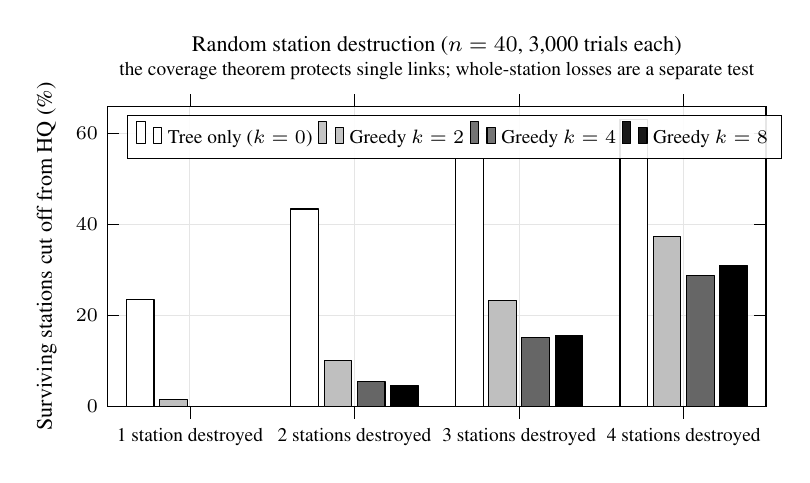
\begin{tikzpicture}
\begin{axis}[width=0.82\textwidth,height=5.4cm,ybar,bar width=10pt,ymin=0,ymax=66,
  title={Random station destruction ($n=40$, 3{,}000 trials each)\\[-1pt]\normalfont\scriptsize the coverage theorem protects single links; whole-station losses are a separate test},
  ylabel={Surviving stations cut off from HQ (\%)},
  xtick={1,2,3,4},xticklabels={1 station destroyed,2 stations destroyed,3 stations destroyed,4 stations destroyed},
  xmin=0.5,xmax=4.5,legend pos=north west,legend columns=4]
  \addplot[fill=white,draw=black] coordinates {(1,23.6)(2,43.4)(3,54.4)(4,63.0)}; \addlegendentry{Tree only ($k=0$)}
  \addplot[fill=black!25,draw=black] coordinates {(1,1.6)(2,10.2)(3,23.3)(4,37.3)}; \addlegendentry{Greedy $k=2$}
  \addplot[fill=black!60,draw=black] coordinates {(1,0.07)(2,5.6)(3,15.3)(4,28.9)}; \addlegendentry{Greedy $k=4$}
  \addplot[fill=black,draw=black] coordinates {(1,0)(2,4.6)(3,15.6)(4,31.0)}; \addlegendentry{Greedy $k=8$}
\end{axis}
\end{tikzpicture}
\caption{Mean percentage of surviving stations cut off from HQ when 1--4 whole stations are destroyed. In the unaugmented
tree, losing one random station cuts off 23.6\% of survivors; greedy cycle backups reduce this to 1.60\% ($k=2$), 0.07\%
($k=4$) and 0.00\% ($k=8$). Multi-station losses show why vertex connectivity and on-demand repair ($E_\text{rec}$) remain
essential.}
\label{fig:station}
\end{figure}

% ==================================================================
\section{Zero-Trust Relaying: AES-256-GCM and Chained HMAC}\label{sec:security}

\subsection{Endpoint payload privacy versus control-plane hop auditing}
Relays in a disaster zone may be physically exposed or untrusted, so SMART-LINK separates endpoint payload encryption from
per-hop route auditing. The origin $v_0$ encrypts plaintext $M$ with AES-256-GCM~\cite{gcm} under a key $K_\text{enc}$ known
only to origin and HQ, a unique 96-bit nonce $N$ (32-bit sender/epoch prefix + 64-bit persistent packet counter) and
immutable additional authenticated data (AAD binding source, destination, session ID and sequence number):
\begin{equation}\label{eq:gcm}
  (C,T_\text{GCM})=\text{GCM-Enc}_{K_\text{enc}}(M,N,\text{AAD}),
\end{equation}
\begin{equation}\label{eq:hmac}
  \tau_i=\text{HMAC-SHA256}_{K_i}\bigl(\mathrm{encode}(\tau_{i-1},R_i)\bigr).
\end{equation}
An analog mixer cannot append bytes by itself; instead each relay's digital control processor parses the unencrypted
routing header and appends a length-delimited canonical hop record $R_i$---binding session ID, packet sequence, relay ID
$v_i$, hop index $i$, outgoing carrier $f_\text{out}$ and a SHA-256 digest of the immutable ciphertext envelope---signed with
a per-relay audit key $K_i$ derived via HKDF~\cite{hmac,hkdf}.

\subsection{Empirical verification}
In \texttt{06\_hmac\_chain.py} the HKDF-SHA256 implementation is first checked against RFC~5869 Test Case~1 (matching the
42-byte OKM bit for bit); we then run 200 adversarial trials for each of eight attack scenarios on a five-hop route
(1{,}600 verifications). Modifying any carrier, deleting an interior hop, swapping two hops or swapping the ciphertext digest
is caught every time (Fig.~\ref{fig:hmac}). The experiment also exhibits two boundaries of the design: (1)~\emph{tail
truncation}---dropping the last hops and presenting the earlier valid tag $\tau_{i-1}$---goes undetected unless HQ checks an
expected final hop count or terminal checkpoint, which restores 100\% detection; and (2)~a \emph{compromised terminal relay}
can sign a false carrier inside its own record $R_i$ with its legitimate key $K_i$. Verification cost is strictly linear in
the hop count, $\approx$9.8\us\ per hop including per-hop HKDF derivation (Fig.~\ref{fig:hmactime}).

\begin{figure}[t]
\centering
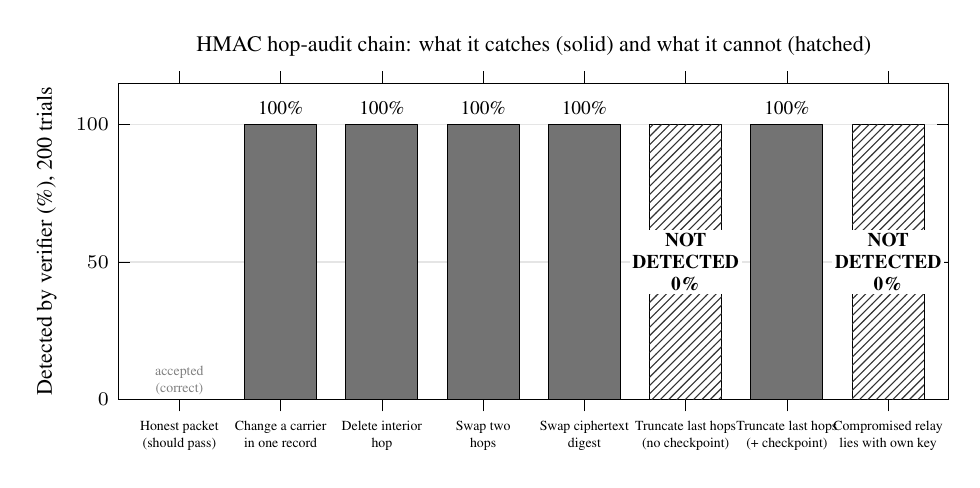
\begin{tikzpicture}
\begin{axis}[width=\textwidth,height=5.6cm,ymin=0,ymax=115,xmin=0.4,xmax=8.6,xtick={1,...,8},
  title={HMAC hop-audit chain: what it catches (solid) and what it cannot (hatched)},
  ylabel={Detected by verifier (\%), 200 trials},
  xticklabels={{Honest packet\\(should pass)},{Change a carrier\\in one record},{Delete interior\\hop},{Swap two\\hops},
    {Swap ciphertext\\digest},{Truncate last hops\\(no checkpoint)},{Truncate last hops\\(+ checkpoint)},{Compromised relay\\lies with own key}},
  xticklabel style={align=center,font=\tiny}, ybar, bar width=26pt, bar shift=0pt, grid=none, ymajorgrids]
  \addplot[fill=black!55,draw=black,nodes near coords={\scriptsize 100\%},every node near coord/.append style={anchor=south}]
    coordinates {(2,100)(3,100)(4,100)(5,100)(7,100)};
  \addplot[fill=white,draw=black] coordinates {(6,100)(8,100)};
  \addplot[pattern=north east lines,pattern color=black!80,draw=none] coordinates {(6,100)(8,100)};
  \foreach \x in {6,8}{\edef\tmp{\noexpand\node[font=\noexpand\scriptsize\noexpand\bfseries,fill=white,inner sep=1pt,align=center] at (axis cs:\x,50) {NOT\\DETECTED\\0\%};}\tmp}
  \node[font=\tiny,text=gray,align=center] at (axis cs:1,7) {accepted\\(correct)};
\end{axis}
\end{tikzpicture}
\caption{Detection rate across eight scenarios (200 trials each). Tampering with any record, hop order or ciphertext digest is
always detected. Tail truncation is detected only with a terminal hop-count checkpoint, and a compromised relay signing a
false value with its own key cannot be detected by the chain alone.}
\label{fig:hmac}
\end{figure}

\begin{figure}[t]
\centering
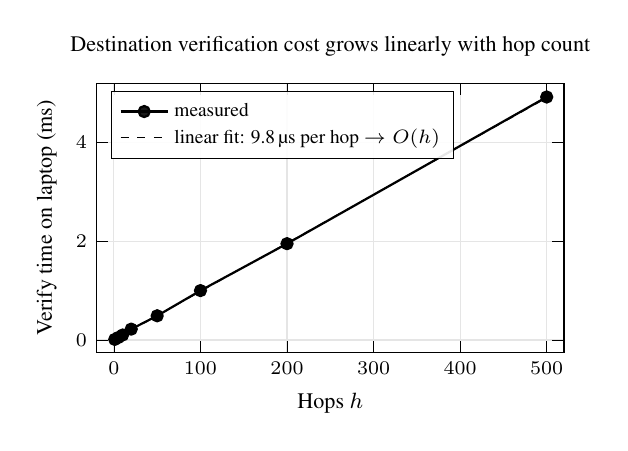
\begin{tikzpicture}
\begin{axis}[width=0.62\textwidth,height=5.0cm,xlabel={Hops $h$},ylabel={Verify time on laptop (ms)},
  title={Destination verification cost grows linearly with hop count},xmin=-20,xmax=520,ymin=-0.25,ymax=5.2,legend pos=north west]
  \addplot[black,thick,mark=*,mark size=2pt] coordinates {(1,0.012)(5,0.05)(10,0.10)(20,0.22)(50,0.49)(100,1.0)(200,1.95)(500,4.92)};
  \addlegendentry{measured}
  \addplot[black,dashed,domain=1:500,samples=2] {0.0098*x+0.003};
  \addlegendentry{linear fit: 9.8\us\ per hop $\rightarrow O(h)$}
\end{axis}
\end{tikzpicture}
\caption{Destination verification time versus hop count $h\in[1,500]$, confirming $O(h)$ verification at $\approx$9.8\us\ per hop
including per-hop HKDF key derivation.}
\label{fig:hmactime}
\end{figure}

% ==================================================================
\section{Algorithmic Complexity}\label{sec:complexity}

Table~\ref{tab:complexity} lists the data structures and asymptotic cost of each pipeline stage. Two practical caveats
matter: the total cached path size $H_P$ can approach $m_0n$, so the greedy stage dominates for large $n$; and under dense
spatial conflicts the number of conflict pairs can reach $J=O(m^2)$.

\begin{table}[h]
\caption{Pipeline stages, data structures and complexity.}\label{tab:complexity}
\footnotesize
\begin{tabularx}{\textwidth}{@{}P{2.5cm}P{4.3cm}P{2.9cm}P{2.4cm}L@{}}
\toprule
\thd{Stage} & \thd{Algorithm \& data structure} & \thd{Time} & \thd{Space} & \thd{Notes}\\
\midrule
1.~Candidate pruning & Spatial grid / $k$-d tree + symmetrized $q$-NN cap ($q=12$) & $O(n^2)$ worst; fast grid average & $O(n+m_0)$, $m_0\le qn$ & Restricted candidate set, not the full radius graph.\\
2.~Backbone tree & Kruskal MST, path-compressed union--find & $O(m_0\log m_0)$ & $O(n+m_0)$ & Spanning forest if $G_0$ is disconnected.\\
3.~LCA path cache & Rooted parent/depth arrays + endpoint-to-LCA climb & $O(n+m_0+H_P)$ & $O(n+m_0+H_P)$ & $H_P=\sum_{\ell\in L}|P_\ell|\le m_0n$.\\
4.~Greedy backups & $k$ exact marginal-gain scans over $L$ & $O(k\cdot H_P)$ & $O(|S|+n)$ & Stops early when the best gain is 0.\\
5.~Bridge detection & Iterative Tarjan low-link DFS & $O(n+m)$ & $O(n+m)$ & Finds uncovered tree edges.\\
6.~Carrier colouring & Degree-ordered first-fit over $r=|\mathcal F|$ carriers and $J=|I|$ conflicts & $O(m\log m+r(m+J))$ & $O(n+m+\Delta(H_c))$ & Dense spatial conflicts: $J=O(m^2)$.\\
7.~Route \& repair & Binary-heap Dijkstra (or BFS) + optional $E_\text{rec}$ pass & $O((n+m)\log n)$ & $O(n+m)$ & $O(1)$ table lookup $\neq$ physical failover latency.\\
\bottomrule
\end{tabularx}
\end{table}

% ==================================================================
\section{Reproducible Software Benchmarks}\label{sec:bench}

All benchmarks use the deterministic Mulberry32 generator with $R_c=0.55$, $q=12$, $s=9$\kHz, $R_I=0.04$ and spatial mode off
by default. On the Seed-42 ten-station baseline ($n=10$, $k=3$), the TypeScript engine (\texttt{src/lib/simulation.ts}) and
the independent Python engine (\texttt{common.py}) both produce 35 candidate links, 9 tree links, greedy backups
$(4,6)$, $(5,7)$, $(0,9)$ with marginal gains $[4,3,2]$, 9/9 protected tree edges, no remaining bridges, $\Delta(G)=4$, and the
four carriers $\{75,84,95,108\}$\kHz---provably minimal since $\chi'(G)\ge\Delta(G)=4$. The figures in this paper were regenerated
from the same stream and reproduce these values exactly. Random $k=3$ selection across 20 seeds (1000--1019) protects a mean of
5.65/9 edges (range 4--8). Table~\ref{tab:scaling} reports scaling to $10{,}000$ stations.

\begin{table}[h]
\caption{Multi-seed scaling (Node.js v24.14.0, AMD Ryzen 7 260).}\label{tab:scaling}
\footnotesize
\begin{tabularx}{\textwidth}{@{}rrrrrrL@{}}
\toprule
\thd{Stations $n$} & \thd{Budget $k$} & \thd{Median (ms)} & \thd{Min--max (ms)} & \thd{Protected links} & \thd{\% protected} & \thd{Interpretation}\\
\midrule
10 & 3 & 0.86 & 0.24 -- 1.98 & 9 -- 9 / 9 & 100.0 & Sub-millisecond; all 9 bridges eliminated.\\
100 & 32 & 5.08 & 3.55 -- 5.27 & 99 -- 99 / 99 & 100.0 & $k=32$ covers all 99 tree edges.\\
1{,}000 & 32 & 83.01 & 60.37 -- 169.98 & 726 -- 751 / 999 & 72.7 -- 75.2 & Interactive ($<0.1$\,s); $\approx$26\% bridges remain.\\
5{,}000 & 32 & 919.27 & 705.15 -- 1{,}505.54 & 2{,}130 -- 2{,}327 / 4{,}999 & 42.6 -- 46.5 & Fixed $k=32$ covers under half the tree.\\
10{,}000 & 32 & 2{,}951.94 & 2{,}364.43 -- 4{,}279.05 & 3{,}373 -- 3{,}632 / 9{,}999 & 33.7 -- 36.3 & $\approx$65\% remain bridges unless $k\propto n$.\\
\bottomrule
\end{tabularx}
\end{table}

A log--log fit of the $n\ge1{,}000$ timings gives $t\propto n^{1.54}$, faster than $n\log n$ because fundamental path lengths, and
hence $H_P$, grow with $n$ (Fig.~\ref{fig:scaling}, left). Holding $k=32$ fixed while $n$ grows to $10{,}000$ drops tree-edge
protection from 100\% to 33.7--36.3\% (right): resilience budgets must scale with network size, e.g.\ $k\approx0.15n$.
Spectrum behaves similarly (Fig.~\ref{fig:carriers}): with station-incidence conflicts only, six carriers always suffice, but
spatial midpoint conflicts ($R_I=0.04$) leave 7.1\% of links unassigned at $n=1{,}000$ and 51.3\% at $n=3{,}000$ as link density
grows inside $[0,1]^2$.

\begin{figure}[t]
\centering
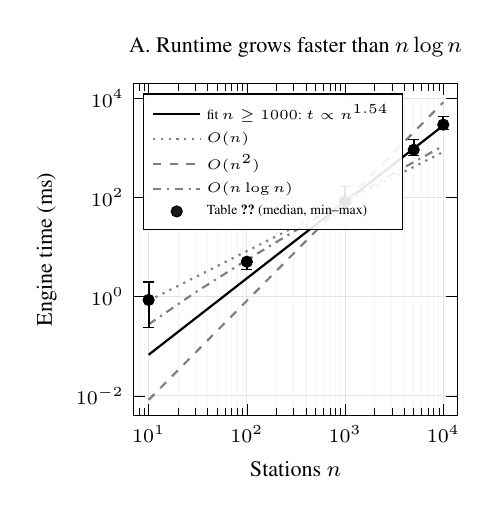
\begin{tikzpicture}
\begin{axis}[width=0.47\textwidth,height=5.8cm,xmode=log,ymode=log,xmin=7,xmax=14000,ymin=4e-3,ymax=2e4,
  title={A.\ Runtime grows faster than $n\log n$},xlabel={Stations $n$},ylabel={Engine time (ms)},
  legend pos=north west,legend style={font=\tiny},minor grid style={gray!8},grid=both]
  \addplot[black,thick] coordinates {(10,0.0675)(10000,2835)}; \addlegendentry{fit $n\ge1000$: $t\propto n^{1.54}$}
  \addplot[gray,thick,dotted] coordinates {(10,0.83)(10000,830)}; \addlegendentry{$O(n)$}
  \addplot[gray,thick,dashed] coordinates {(10,0.0083)(10000,8300)}; \addlegendentry{$O(n^2)$}
  \addplot[gray,thick,dashdotted] coordinates {(10,0.2767)(30,1.226)(100,5.533)(300,20.55)(1000,83)(3000,295.5)(10000,1106.7)}; \addlegendentry{$O(n\log n)$}
  \addplot[black,only marks,mark=*,mark size=2pt,error bars/.cd,y dir=both,y explicit,error bar style={thick}]
    coordinates {(10,0.86) += (0,1.12) -= (0,0.62)
                 (100,5.08) += (0,0.19) -= (0,1.53)
                 (1000,83.01) += (0,86.97) -= (0,22.64)
                 (5000,919.27) += (0,586.27) -= (0,214.12)
                 (10000,2951.94) += (0,1327.11) -= (0,587.51)};
  \addlegendentry{Table~\ref{tab:scaling} (median, min--max)}
\end{axis}
\end{tikzpicture}\hfill
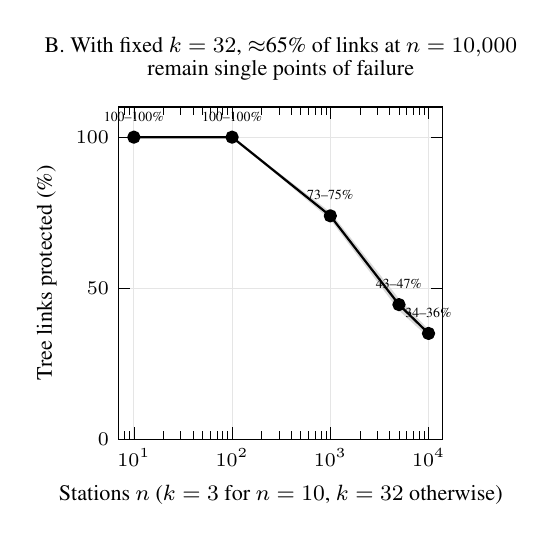
\begin{tikzpicture}
\begin{axis}[width=0.47\textwidth,height=5.8cm,xmode=log,xmin=7,xmax=14000,ymin=0,ymax=110,
  title={B.\ With fixed $k=32$, $\approx$65\% of links at $n=10{,}000$\\[-1pt]remain single points of failure},
  xlabel={Stations $n$ ($k=3$ for $n=10$, $k=32$ otherwise)},ylabel={Tree links protected (\%)}]
  \addplot[fill=black!15,draw=none] coordinates {(10,100)(100,100)(1000,72.7)(5000,42.6)(10000,33.7)(10000,36.3)(5000,46.5)(1000,75.2)(100,100)(10,100)} -- cycle;
  \addplot[black,thick,mark=*,mark size=2pt,
    nodes near coords, point meta=explicit symbolic, every node near coord/.append style={font=\tiny,anchor=south,yshift=2pt}]
    coordinates {(10,100)[100--100\%] (100,100)[100--100\%] (1000,73.95)[73--75\%] (5000,44.55)[43--47\%] (10000,35.0)[34--36\%]};
\end{axis}
\end{tikzpicture}
\caption{Re-analysis of the scaling table. Left: log--log fit of Table~\ref{tab:scaling} execution times, showing empirical
$t\propto n^{1.54}$ for $n\ge1{,}000$ against $O(n)$, $O(n\log n)$ and $O(n^2)$ references anchored at $n=1{,}000$. Right: with
$k=32$ fixed, tree-edge protection falls from 100\% to 33.7--36.3\% (band = min--max over seeds).}
\label{fig:scaling}
\end{figure}

\begin{figure}[!htb]
\centering
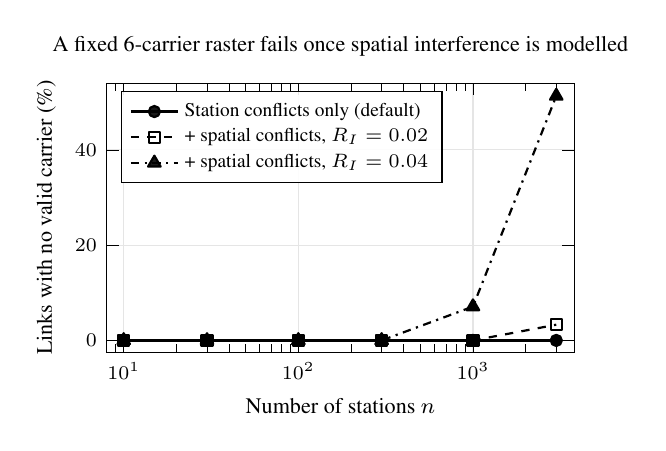
\begin{tikzpicture}
\begin{axis}[width=0.62\textwidth,height=5.0cm,xmode=log,xmin=8,xmax=3800,ymin=-2.5,ymax=54,
  title={A fixed 6-carrier raster fails once spatial interference is modelled},
  xlabel={Number of stations $n$},ylabel={Links with no valid carrier (\%)},legend pos=north west]
  \addplot[black,thick,mark=*,mark size=2pt] coordinates {(10,0)(30,0)(100,0)(300,0)(1000,0)(3000,0)};
  \addlegendentry{Station conflicts only (default)}
  \addplot[black,thick,dashed,mark=square,mark size=2pt,mark options={solid}] coordinates {(10,0)(30,0)(100,0)(300,0)(1000,0)(3000,3.3)};
  \addlegendentry{+ spatial conflicts, $R_I=0.02$}
  \addplot[black,thick,dashdotted,mark=triangle*,mark size=2.6pt,mark options={solid}] coordinates {(10,0)(30,0)(100,0)(300,0)(1000,7.1)(3000,51.3)};
  \addlegendentry{+ spatial conflicts, $R_I=0.04$}
\end{axis}
\end{tikzpicture}
\caption{Percentage of links left without a valid carrier as $n$ scales from 10 to 3{,}000. Six carriers suffice for
station-incidence conflicts; spatial midpoint conflicts at $R_I=0.04$ leave 7.1\% unassigned at $n=1{,}000$ and 51.3\% at
$n=3{,}000$.}
\label{fig:carriers}
\end{figure}

% ==================================================================
\section{Raspberry Pi Pico Hardware-in-the-Loop Testbench}\label{sec:hw}

We distinguish physical RF full-duplex cancellation, which needs specialized RF front-end hardware, from the Raspberry Pi Pico
(RP2040) testbench (\texttt{pico/pico\_node.py}). Using three or four Pico boards, the testbench executes the real digital control
plane and makes frequency translation audible:
\begin{itemize}\setlength\itemsep{1pt}
  \item \textbf{Embedded HKDF + chained HMAC-SHA256.} Each Pico derives its relay key $K_i$ by RFC~5869 HKDF, parses incoming JSON
        packets over UART1 (115{,}200\,baud), computes Eq.~\eqref{eq:hmac} with a canonical fixed-order byte encoding, and logs
        processing latency in microseconds (\texttt{time.ticks\_us()}).
  \item \textbf{Audible carrier translation.} Each Pico drives a piezo buzzer on GP15 at its assigned carrier scaled by $1/100$ into
        the audio band (75\kHz$\to$750\,Hz, 84$\to$840\,Hz, 95$\to$950\,Hz, 108$\to$1{,}080\,Hz), so each hop's frequency shift can be heard.
  \item \textbf{Interactive tamper button (GP13).} Holding the button on any relay injects a live man-in-the-middle attack (mutating
        the outgoing carrier metadata to $f_\text{out}=1350$ after HMAC tagging). The destination Pico immediately extinguishes its
        green verification LED (GP14) and reports \texttt{verified=0} over USB serial.
\end{itemize}

\begin{table}[!htb]
\caption{Four-Pico daisy-chain wiring and pinout.}\label{tab:pico}
\footnotesize
\begin{tabularx}{\textwidth}{@{}P{2.0cm}P{2.3cm}P{3.4cm}P{3.6cm}L@{}}
\toprule
\thd{Board / role} & \thd{Node ID \& carrier} & \thd{UART1 data wiring} & \thd{Peripherals (GP13--15)} & \thd{Action}\\
\midrule
Pico 0: origin & \texttt{NODE\_ID=0}, 750\,Hz & GP4 (TX) $\to$ Pico~1 GP5 (RX); common GND & GP14 TX LED; GP15 750\,Hz buzzer & Generates packet + initial session tag $\tau_0$ every 200\,ms.\\
\lightrule
Pico 1: relay 1 & \texttt{NODE\_ID=1}, 840\,Hz & GP5 (RX) $\leftarrow$ Pico~0 GP4; GP4 (TX) $\to$ Pico~2 GP5 & GP13 tamper switch to GND; GP14 hop LED; GP15 840\,Hz & Appends $R_1$, updates $\tau_1$; hold GP13 to tamper.\\
\lightrule
Pico 2: relay 2 & \texttt{NODE\_ID=2}, 950\,Hz & GP5 (RX) $\leftarrow$ Pico~1 GP4; GP4 (TX) $\to$ Pico~3 GP5 & GP13 tamper switch to GND; GP14 hop LED; GP15 950\,Hz & Appends $R_2$, updates $\tau_2$, measures hop time.\\
\lightrule
Pico 3: HQ & \texttt{NODE\_ID=99}, USB serial & GP5 (RX) $\leftarrow$ Pico~2 GP4; USB to laptop & GP14 green verify LED; CSV \texttt{seq,hops,verified,us} & Recomputes the $O(h)$ chain; lights LED iff valid.\\
\bottomrule
\end{tabularx}
\end{table}

\noindent The relay audit loop at the core of \texttt{pico\_node.py} is:
\begin{lstlisting}
def encode(prev, rec):  # canonical fixed-order encoding (immune to dict key ordering)
    body = '{}|{}|{}|{}|{}|{}'.format(rec['s'], rec['q'], rec['r'], rec['h'], rec['f'], rec['ct']).encode()
    return len(prev).to_bytes(4, 'big') + prev + len(body).to_bytes(4, 'big') + body

# inside the RELAY loop, on receiving a packet over UART1:
t_start = time.ticks_us()
rec = {'s': SESSION, 'q': pkt['seq'], 'r': NODE_ID, 'h': len(pkt['hops']) + 1, 'f': CARRIER_HZ, 'ct': pkt['ct'][:16]}
tau = hmac_sha256(K, encode(ubinascii.unhexlify(pkt['tau']), rec))
if not evil.value(): rec['f'] = 1350   # GP13 tamper switch pressed -> corrupt carrier after signing
rec['us'] = time.ticks_diff(time.ticks_us(), t_start)
pkt['hops'].append(rec); pkt['tau'] = ubinascii.hexlify(tau).decode(); send(pkt)
\end{lstlisting}

\begin{keybox}{From UART jumper wires to true multi-frequency RF}
To demonstrate wireless multi-channel failover, an nRF24L01+ (2.4\,GHz SPI transceiver, about INR~150) or SX1278 LoRa (433\,MHz)
module can be attached to each Pico's SPI0 pins (GP16--GP19), mapping SMART-LINK's assigned carrier $f_e$ directly to
\texttt{nrf.set\_channel(ch)}.
\end{keybox}

% ==================================================================
\section{Limitations}\label{sec:limits}

\begin{itemize}\setlength\itemsep{1pt}
  \item \textbf{Restricted candidate graph.} Coverage guarantees and MST optimality hold relative to the symmetrized $q$-NN graph
        $G_0$ ($R_c=0.55$, $q=12$); full radius graphs or terrain-obstructed deployments can yield different topologies.
  \item \textbf{Single-link versus multi-failure resilience.} Theorem~\ref{thm:greedy} protects weighted tree edges against single-link
        cuts. Simultaneous multi-link cuts, articulation-station losses and correlated disasters require higher vertex
        connectivity or spare candidate links via on-demand repair ($E_\text{rec}$).
  \item \textbf{Centralized recolouring.} The playground recomputes carrier assignments globally; field deployment requires a
        distributed control channel and a transition handshake.
  \item \textbf{RF and cryptographic deployment.} The suite verifies the FFT and Butterworth response, the link-budget equations
        and the HKDF + HMAC tamper matrix; operational full-duplex cancellation ($>140$\,dB from $+30$\,dBm TX to a $-110$\,dBm
        floor), key provisioning, persistent nonce state and terminal hop-count checkpoints remain deployment requirements.
\end{itemize}

\section{Conclusion}\label{sec:conclusion}

SMART-LINK shows that a disaster network's cost, resilience, spectrum and trust can be engineered in one transparent
pipeline. Cycle coverage is submodular, so a simple greedy rule protects at least 63.2\% of what an optimal budgeted design
could---and in practice matches it in 96.78\% of scenarios. Carrier assignment is a list $T$-colouring that meets Vizing's
lower bound on small networks but saturates a fixed raster under dense spatial interference; analog relaying is fast
(159.1\us\ per hop) but capped at $\approx$8\,kbit/s in a 4\kHz\ passband and accumulates noise; and an HMAC hop chain catches
every in-path modification provided HQ checks the terminal hop count. Each of these claims is reproduced by the open
simulation suite and the RP2040 testbench, and each comes with an explicit boundary of validity.

% ==================================================================
\clearpage
\begingroup
\renewcommand\refname{References}
\small
\begin{thebibliography}{9}\setlength\itemsep{1pt}
\bibitem{nemhauser} G.~L. Nemhauser, L.~A. Wolsey, and M.~L. Fisher, ``An analysis of approximations for maximizing submodular
  set functions---I,'' \emph{Mathematical Programming}, vol.~14, pp.~265--294, 1978. doi:10.1007/BF01588971.
\bibitem{bharadia} D.~Bharadia, E.~McMilin, and S.~Katti, ``Full duplex radios,'' in \emph{Proc. ACM SIGCOMM}, pp.~375--386, 2013.
  doi:10.1145/2486001.2486033.
\bibitem{vizing} V.~G. Vizing, ``On an estimate of the chromatic class of a $p$-graph,'' \emph{Diskret. Analiz}, no.~3, pp.~25--30, 1964.
\bibitem{smida} B.~Smida, R.~Wichman, K.~E. Kolodziej, H.~A. Suraweera, T.~Riihonen, and A.~Sabharwal, ``In-band full-duplex: The
  physical layer,'' \emph{Proceedings of the IEEE}, vol.~112, no.~5, pp.~433--462, 2024. doi:10.1109/JPROC.2024.3366768.
\bibitem{gcm} M.~Dworkin, \emph{Recommendation for Block Cipher Modes of Operation: Galois/Counter Mode (GCM) and GMAC}, NIST
  SP~800-38D, Nov.~2007. doi:10.6028/NIST.SP.800-38D.
\bibitem{hmac} H.~Krawczyk, M.~Bellare, and R.~Canetti, ``HMAC: Keyed-hashing for message authentication,'' RFC~2104, Feb.~1997.
\bibitem{hkdf} H.~Krawczyk and P.~Eronen, ``HMAC-based extract-and-expand key derivation function (HKDF),'' RFC~5869, May~2010.
\bibitem{smartlink} Thishyaketh~A., Abhayavarman~B., V.~E. Ilam Barathi, S.~Madhavan, Shiddheesh~K., and R.~Jaiprajen,
  ``SMART-LINK: Resource-constrained network resilience'' (design paper, \texttt{SMART-LINK-Final.pdf}), RSBVP 2026--27, 2026.
\end{thebibliography}
\endgroup

% ==================================================================
\appendix
\section{Equation Summary}\label{app:eqs}

\begin{table}[h]
\footnotesize
\begin{tabularx}{\textwidth}{@{}P{0.9cm}P{2.6cm}L@{}}
\toprule
\thd{Eq.} & \thd{Layer} & \thd{Statement and scope}\\
\midrule
\eqref{eq:dist} & Candidate graph & $d(i,j)=\sqrt{(x_i-x_j)^2+(y_i-y_j)^2}$, retaining symmetrized top-$q$ neighbours within $R_c$.\\
\eqref{eq:cov} & Cycle coverage & $\mathrm{Cov}(S)=\bigcup_{\ell\in S}P_\ell$, $F(S)=\sum_{e\in\mathrm{Cov}(S)}w_e$, $\max_{|S|\le k}F(S)$.\\
\eqref{eq:gain} & Marginal gain & $F(A\cup\{\ell\})-F(A)=\sum_{e\in P_\ell\setminus\mathrm{Cov}(A)}w_e$, nonincreasing in $A$ $\Rightarrow$ submodular.\\
\eqref{eq:bound} & Greedy guarantee & $F(S_g)\ge[1-(1-1/k)^k]F(S^\ast)\ge(1-1/e)F(S^\ast)$ for fixed $L$ and $w_e\ge0$.\\
\eqref{eq:gap} & Submodular gap & $F(S^\ast)-F(S_t)\le\sum_{\ell\in S^\ast\setminus S_t}[F(S_t\cup\{\ell\})-F(S_t)]$.\\
\eqref{eq:conflict} & Conflict graph & $A_{e,e'}=1$ if $e\cap e'\ne\emptyset$ or (spatial mode and $\|m_e-m_{e'}\|_2\le R_I$).\\
\eqref{eq:sep} & Carrier separation & $f_e\in L_e=\mathcal F\setminus J_e$, $|f_e-f_{e'}|\ge s$ for every $\{e,e'\}\in I$.\\
\eqref{eq:guard} & Guard-band rule & $|f_e-f_{e'}|\ge(B_e+B_{e'})/2+g_{e,e'}$.\\
\eqref{eq:mix} & Heterodyne mixer & $y_\text{mix}=a\cos(2\pi(f_\text{in}-f_\text{LO})t+\phi)+a\cos(2\pi(f_\text{in}+f_\text{LO})t+\phi)$.\\
\eqref{eq:leak} & Leakage budget & $P_\text{residual}=P_\text{tx}-A_\text{antenna}-A_\text{filter}-A_\text{cancellation}$.\\
\eqref{eq:sinr} & Physical SINR & $\mathrm{SINR}_e=P_eg_e/(N_0B_e+\sum_{j\ne e}P_jg_{j\to e}\eta_{j,e})$; $C_e=B_e\log_2(1+\mathrm{SINR}_e)$.\\
\eqref{eq:route} & Shortest routing & $Q^\ast\in\arg\min_{Q\subseteq E_\text{usable}}\sum_{e\in Q}c_e$ (or $\min|Q|$ in BFS mode).\\
\eqref{eq:repair} & Corridor repair & $E_\text{rec}=Q_0\setminus(E_T\cup S)$, prioritized during recolouring after severe outages.\\
\eqref{eq:gcm} & Endpoint GCM & $(C,T_\text{GCM})=\text{GCM-Enc}_{K_\text{enc}}(M,N,\text{AAD})$, unique 96-bit nonce, 128-bit tag.\\
\eqref{eq:hmac} & Relay HMAC chain & $\tau_i=\text{HMAC-SHA256}_{K_i}(\mathrm{encode}(\tau_{i-1},R_i))$, HKDF-derived $K_i$.\\
\bottomrule
\end{tabularx}
\end{table}

\end{document}
